\documentclass{article}
\usepackage[a4paper, left=35mm, right=35mm]{geometry}

%Spaced paragraphs instead of indentation
\usepackage[parfill]{parskip}

%Fonts
\usepackage{fontspec}
\setmainfont{Rene_Bieder_-_Galano_Grotesque}[
Path = Galano_Grotesque_Family/,
Extension = .otf,
UprightFont = *_Regular,
BoldFont = *_Bold,
ItalicFont = *_Italic,
BoldItalicFont = *_Bold_Italic
]

%To redefine titles/sections and their shapes.
\usepackage{titlesec}
\titleformat{\paragraph}[runin]{\bfseries\small}{\theparagraph}{1em}{}[\hspace{0.5em}-]
\titlespacing*{\paragraph}{0pt}{0.5em}{0.5em}
\newcommand{\sectionbreak}{\clearpage}


\usepackage[style=numeric]{biblatex} %Reference managment
\addbibresource{references.bib}
\usepackage[english]{babel} %Languages
\usepackage{csquotes} %Recommended to use with babel


\usepackage{graphicx} %For images
\graphicspath{ {./images/} }

\usepackage[justification=centering]{caption} % To center captions

\usepackage{svg} %To handle include of SVG type images

\usepackage{float} % for [H] option in figures
\usepackage{wrapfig} %figures wrapped in text

%Center all floats
\makeatletter
\g@addto@macro\@floatboxreset\centering
\makeatother

\usepackage{array} %Lets set tabular extrarowheight
\usepackage{amsmath} %Cool maths

\usepackage[font=small,labelfont=bf]{caption} %Better captions for figures and tables

%\usepackage{footnote} %For footcite in figure caption

\usepackage{xcolor} %Add colours

%Use more links and modify their looks. Apparently also meta data
\usepackage{hyperref}
\hypersetup{
	pdftex,
	pdftitle={Predictive model for Traffic Control in Undegeround Mines},
	pdfauthor={Claes Andersson},
	pdfsubject={Underground Mine Traffic Control}, % What is this supposed to be????
	pdfkeywords={Underground, Mines, Tunnels, Traffic, Control, Management, System, Collision Avoidance, Single track}
}

\hypersetup{
    colorlinks,
    linkcolor={black!50!black},
    citecolor={black!50!black},
    urlcolor={black!80!black}
}


\begin{document}
    \begin{titlepage}


        % \title{Predictive model for Traffic Control in Undegeround Mines}
        % \author{Claes Andersson \\ Mobilaris MCE}
        % \maketitle

        \begin{abstract}
			Due to the nature of tunnels, a driver in an underground mine may find themselves driving without much vision of the road up ahead. The tunnels usually allow for traffic in both directions but are often only wide enough for a single vehicle. To let vehicles pass each other meeting slots have been carved into the tunnel walls, where one can park while the other passes. Because of the limited vision, however, it is unlikely that a meeting with another vehicle will occur directly next to such a meeting slot. Instead, one of the vehicles must reverse to the closest meeting slot in order to let the other pass. This makes mine tunnels a very inhospitable driving environment, causing disruptions to traffic flow throughout the mine. Unfortunately, typical traffic management or scheduling solutions are not useful, as real-time positioning for the vehicles is often poor while network connectivity cannot be guaranteed in the mine environment.

			This thesis presents a solution which will avoid situations where a driver needs to back up, and instead present meeting slots in which to park ahead of time. This is done by calculating velocity probability distributions for road segments from historical data and using these to estimate arrival times to meeting slots. In addition, a more comprehensive solution is presented, taking into account the accuracy of positioning, outdated information due to poor connections and more complicated scenarios.

			The results show that estimating arrival times using only historical data is a very feasible technology, which can realistically be implemented today. Such an implementation could, in the author's opinion, improve driver safety and efficiency significantly, compared to a driver having no information or simply knowing rough positions of nearby vehicles. This being said, there are still steps that can be taken to improve the solution and to develop a more comprehensive system overall.

        \end{abstract}

        \thispagestyle{empty}
    \end{titlepage}

		\setcounter{secnumdepth}{3}
		\setcounter{tocdepth}{3}
		\tableofcontents
		\newpage

    \section{Introduction}
		An underground mining operation is a complex operation. It requires a lot of people and vehicles to travel up and down the mine at various times, as well as back and forth inside the mine itself. The actual tunnelling, though, is a very expensive undertaking, and despite the existence of numerous vehicles a vast majority of underground mining tunnels are only wide enough to accommodate a single vehicle. Vehicles must still be able to pass each other, and therefore meeting slots are spaced out along road segments to allow vehicles to park and make way for others to pass. Winding roads do not allow for a good line of sight, unfortunately, and as such drivers will not know what oncoming traffic they have. Without any assistance a driver will traverse a tunnel until a meeting of a vehicle travelling the opposite direction occurs. The distance at which two drivers detect each other might be very short due to the limited vision. At the point of contact the drivers of both vehicles must decide who must back up and make way. For some vehicles it is of utmost importance that they never stop at all, such as fully loaded trucks heading up and out of the mine, since they might stall and be unable to restart if stopped. Resolving such a situation can take time, stall heavy vehicles, cost production time, and resources, as well as be very stressful for the drivers involved. Additionally, reversing on a narrow road and around corners might result in accidental vehicle damage if accidentally reversing into a wall or obstacle.

		A favourable option would be for the drivers of each vehicle to be provided with technological solutions that present more information and could suggest a course of action that would avoid head-on meetings with other vehicles, and thus eliminate the need to reverse through narrow passageways. The purpose of this master's thesis is to develop such a solution.

		However, a hindrance to such a solution is that the thick layer of rock overhead in an underground mine blocks any radio signals from penetrating down to the vehicles. This means that any satellite-based geopositioning systems, such as GPS, is impossible to use. Communication within the mine suffers the same issue of impenetrable rock, and as a consequence many mines install WiFi throughout the mine. Such a WiFi system can be used for positioning in addition to communication, and thus alleviates the issue of not having GPS. Unfortunately, everything has its costs, including connectivity. It is not unlikely that a system has its infrastructure nodes placed with quite large distances apart, and therefore connectivity  to the WiFi system can in places be very unreliable. Thus, WiFi positioning inside a mine can be quite inaccurate, down to an accuracy of barely 100m precision \cite{Gronlund}. Accuracy can be improved by installing more advanced infrastructure or solutions, for example Ultra Wide Band, UWB. It could be the case that several systems are in use, with important parts of the mine be fitted with UWB infrastructure, very important vehicles be fitted with sensors and algorithms, and the rest be left to rely on WiFi positioning only. Regardless of which, no system is perfect, and a lot of uncertainty is involved in the positioning of vehicles.

		\subsection{Problem description}
			This thesis will address the problem of two vehicles unknowingly travelling towards each other down the same segment of road from opposite ends, and thus meeting each other head-on in the middle, not permitting either to continue and forcing one of them to reverse. From here on this is referred to as a `collision'. Collisions can be avoided by one vehicle giving way, either by parking in a meeting slot or diverging down a different road. Since connectivity is not guaranteed at all times the solution algorithm must be able to run independently on every vehicle.

			This problem can be broken down into several subproblems
			\begin{itemize}
				\item Identify oncoming vehicles
				\item Identify nearby meeting slots or places to give way
				\item Predict difference in arrival time to a meeting slot
				\item Manage inaccurate positioning
				\item Manage loss of connection and old data
			\end{itemize}

			The specifics of identifying oncoming vehicles and meeting slots is implementation specific and not important. This master's thesis will focus on predicting difference in arrival time to any point in the map and managing inaccurate positioning and connections. Predicting difference in arrival time to a meeting slot means that given two vehicles and a point in between them a prediction is made for each vehicle of how long time it will take to reach the given point. Poor prediction of arrival times could result in either suggestions for a vehicle to wait at a meeting slot which is not the optimal solution, and thus slow down traffic and decrease efficiency, or result in a collision and the need for one of the vehicles to reverse.

			The resources available to use in order to solve the problem are:
	        \begin{itemize}
                \item A graph map of the mine layout .
                \item A position for every vehicle in the mine with a given accuracy rating and timestamp.
				\item History of previous travel in form of logs.
	            \item An onboard computer in every vehicle that runs the solution algorithm
	            \item Known destinations and routes for each vehicle.
	        \end{itemize}

			The mine map can easily be transferred to an onboard computer and kept in memory, and can thus be used effortlessly by the vehicle computer.

			With the listed resources collisions will be avoided as best as possible. To this end, the solution algorithm must present drivers with upcoming collisions and one or more solutions to the collision so that it can be prevented. With perfect system knowledge the solution algorithm should prevent all collisions. The information regarding positioning and their accuracies is continuously updated, and as such the solution algorithm must be lightweight enough to run frequently, in the range of once every few seconds at least. Thus the aim is to create an algorithm based on heuristics, as providing an exhaustive exploration of the problem space would not be suitable for real-time use.

			It will also be assumed that all vehicles in the system uses the solution algorithm and follows its instructions.

			\subsubsection{Challanges}
				The two major hurdles are inaccurate positioning and unreliable WiFi connections. Inaccurate positioning means that one can seldom be entirely sure where a given vehicle actually is. A vehicle can not even be entirely sure of its own position. This is compounded by unreliable WiFi connections, which means that positional data from other vehicles might be old since the connection to the network cannot be guaranteed. These two things contribute to uncertainty, which is the main problem in this algorithm solution. Since uncertainty is most likely not equal to zero, there is always a risk involved in any collision avoidance. At some point it must be decided what risk one is willing to take. Taking no risk at all would reduce the overall number of collisions while decreasing overall flow and so might decrease production. Taking some risk might increase flow, but also the number of collisions.

			% \subsubsection{Problems}
			% 	The conditions assumed and problems the suggested solution will operate under are listed here.
				The problems the suggested solution will operate under are summarized as
				\paragraph{Risks}
					Vehicles should ideally never collide, but an accepted risk of collision can be defined.
				\paragraph{Single lane}
					All road segments in the mine will be assumed to be single lane. No passing is possible unless one vehicle gives way at a junction or in a meeting slot.
				\paragraph{Connectivity}
					Connectivity is assumed to be shaky, and at some points non-existent.
				\paragraph{Accuracy}
					Accuracy can range from great to poor.
				\paragraph{Prioritized}
					Some vehicles are prioritized higher than others. A vehicle with lower priority needs to give way to one with a higher priority.

			\subsubsection{Delimitations}
				This thesis is entirely concerned with the avoidance of collisions in the mine. Many other metrics can be important in a mine, and might even be more important than avoiding collisions, such as overall traffic flow, production output, inclined vs declined driving, entering vs exiting vehicles, fuel usage, etc. Such things are not considered, however.

				The remainder of this subsection is a collection of the conditions and problems that this master's thesis will not attempt to address. Like with metrics, many of these problems are very relevant in a real world scenario, but add little value to the central problem and simply add more irrelevant edge cases. They may vary depending on the mine in which they are used, and dealing with them is thus left to the discretion of any real-world implementation.
				\paragraph{Dual lane}
					While they exist in some mines, they will not be included in this thesis.
				\paragraph{Passing}
					Fast vehicle being allowed to pass slower ones to increase flow will not be a criteria.
				\paragraph{People}
					While they exist and can be positioned in mines, they are an edge case that will not be included. Vehicles are the main focus.
				\paragraph{Advanced pathing}
					The solution will not try to find a better route around if multiple paths are available.
				\paragraph{Non-conformity}
					The thesis will not address vehicles in the system that do not follow the suggestions of the solution algorithm in some way, or that do not use it at all.
				\paragraph{Execution time}
					This thesis will not examine execution time on the expected usage systems under expected load.
				\paragraph{Priority calculation}
					Priority will be assumed to have been assigned to every vehicle prior to the solution algorithm being run. This thesis will not deal with determining what base priority any vehicle has.
				\paragraph{Equal priority}
					As an extension of the previous point, this thesis will not address the problem of vehicles having the same priority.


		\subsection{Technologies}
			Mobilaris MCE AB, referred to simply as Mobilaris in this thesis, is the sponsor of this thesis. %owner of this thesis.
			Although the concepts and solutions described in this thesis do not depend on any Mobilaris products per se, assumptions on available technology and restrictions are made based on those that would exist in a mine fully equipped with Mobilaris products. Later in this thesis testing data is collected from Mobilaris technologies and used to evaluate the solution. Therefore technologies needed, and some relevant Mobilaris solutions are briefly explained here.

			Knowledge of the mine layout is needed and is naturally represented in the form of a graph. In this thesis the mine map data structure will be a \textit{doubly connected edge list}, DCEL, \cite{ComputationalGeometry} in which faces are disregarded. The nodes of the graph are arbitrary points along the mine road network, spaced out to give suitable granularity. In this thesis, this granularity is slightly less than five meters. The edges of the data structure are the road segments spanning between nodes.

			A system for positioning inside the mine is needed for two reasons. The main reason being, of course, to acquire a rough position of where vehicles are inside the mine for use in the algorithm. The second reason being to build up a history of traversals throughout the mine. There are several systems which could fill this role, such as UWB, WiFi, RFID, to give some examples. This thesis uses the positioning and data generated by Mobilaris' proprietary system \textit{Mobilaris Hybrid Positioning\texttrademark}, Hybrid Positioning for short, which uses WiFi, sensors, and knowledge of the mine to determine a position. This is all done on a tablet installed in the vehicle, and the system has an alleged accuracy of around five to ten meters \cite{MobilarisHybridP}, although there is no published study to back this up. The use of this system is also the reason why the granularity of the mine map nodes is chosen to be around five meters. The solution proposed is however intended to work with different positioning systems being in use at the same time, with varying degrees of accuracy.

			To present information and to run the algorithm itself some sort of computer is needed in vehicles installed with the system. Mobilaris uses a tablet for their solutions which is also the intended target system for this thesis. Today, a Mobilaris equipped tablet can display the rough distance of close-by vehicles, however it does not direct the driver to meeting slots nor predict collisions. Regardless of the type of computer it would need to be able to communicate to the network. In this thesis, this is assumed to be done over WiFi.

			Logs of historical travel data need to retell how fast vehicles travel throughout the mine. The logs used in this thesis comes from the Hybrid Positioning system, which logs the state of position and velocity at given timestamps. The velocity state in the Hybrid Positioning system is provided by On-board diagnostics, OBD, \cite{obd} which is a system built into most vehicles for reading data about the vehicle.

    	\subsection{Related work}
			The field of traffic management in underground mines is not very well explored and related works can be hard to come by. This can mainly be attributed to the lack of generalised positioning systems with adequate accuracy to allow for such a system. The problem space is quite analogous to train routing on single tracks, though. For two trains to meet head-on is very undesirable, they have side tracks and stations to wait at for a clear track. However they do not have to deal with risks in the same way, as their speed traversing the track is more or less known and predetermined, and their position can be determined quite easily. In general, this can be seen as a scheduling problem on a single lane.

			In this sections ``this master's thesis'' will refer to this very thesis, while ``the paper'' will refer to the work last referenced.

			Varandas et al. \cite{BadPaper} describe a system trying to solve the problem of vehicle collisions in underground mines, the same as this master's thesis. What is described is a very simplistic solution, relying on traffic lights throughout the managed area and very coarse positioning. The accuracy of the positioning system is never specified, and sources for the characteristics specified are never given. Despite this, precision can be assumed to be very poor based on the technological landscape of 2014 and the experiences gained by Mobilaris. The paper also allows for a halt order to be given to a vehicle with absolute priority in the spirit of avoiding collisions. The efficacy of the system is never proven or addressed. Seems to be an advertisement in disguise as a research paper. In contrast to Varandas et al. this master's thesis will always preserve priority. If two vehicles are poised to collide the lower priority one will always be forced to back, even if the higher priority vehicle could park or stop to prevent the collision.

			Åhlén \cite{UppsalaPaper} addresses the same issue of traffic management in underground mines as well. In this paper, path-finding and collision avoidance is explored thoroughly and ensures that priority is never betrayed unless absolutely necessary. The methodology is tested through simulation, however the actual results are somewhat vague. The paper does not have any real-world data with which to back their findings up with, unfortunately, and the simulation is a simplification in many regards. For instance, positions of vehicles are perfectly known, and the velocity at which they travel over edges are known constants. Despite this, the methodology for collision avoidance employed seem very well thought out.

			Xu et al. \cite{TrainPaper} addresses time tabling of trains, and how to determine track clearance for single-track railway systems. A train track pass provides the possibility for two trains to travel parallel to each other while passing, and in such provide a flow for both directions at the same time. The use case of this master's thesis is somewhat different in that one of the two vehicles have to remove themselves from the road segment and park away while the other passes. Thus a lot of scenarios are quite differenet. Xu et al. do not have to contend with unknown positioning either and it is assumed that position is fairly well known.

%			de Oliveira \cite{JobShopSchedule} defines a similar problem in the train scheduling space as a Job Shop Scheduling problem, which is an NP-complete problem. . This master's thesis will differ in that it will solve the issue using heuristics, and as such not be NP-complete. As a consequence the solutions will not always be optimal, however optimal solutions are unobtainable with inaccurate positioning regardless.

		\subsection{Contribution}
			As previously stated the solution must be lightweight and run frequently on a tablet and thus will be using heuristics instead of solving an NP-complete scheduling problem optimally. One idea would be to use machine learning to try to produce a system that avoids collisions by punishing collisions and delays. However, due to the complexity of the problem depending on so many variables and mine layout, and the author's lacking experience in machine learning, this approach was turned down.

			In contrast, the spirit of the algorithm devised by Xiaoming Xu et al. seems like quite an appropriate fit, where every vehicle looks ahead and determines the clearance for continued traversal. Although, a system-wide solution for the entire traversal of every vehicle cannot be produced as drivers in a mine cannot really be held to a timetable, and since the uncertainties involved would quickly break down such a scheduling. However, planning for the immediate future can be done. All positioning is uncertain, as is traversal speed, and is subject to probability distributions. This master's thesis will attempt to produce a solution that deals with the uncertain nature of the problem, plan for the immediate future for a vehicle and provide the best solution for avoiding collisions with a given probability of success.

    \section{Theory}
		This section will suggest a solution to the presented problem of avoiding collisions in a mine. The overarching idea is to use historical logs to predict velocity for vehicles, and using this velocity and distance from a vehicle to a point to estimate the arrival times for a vehicle to that point. When estimating the arrival time of two vehicles to the same point it can be predicted which vehicle will arrive first. If the chosen point is a meeting slot then a driver on a collision course can be informed of which meeting slot to park in and the chance of making it there without a collision is.

		\subsection{Velocity probability distribution}
			An underground mine can present a lot of different conditions for a traversing vehicle. One could find winding slopes as well as long flat straights, great road quality in some places and very poor in others. Therefore one can assume that different road segments in the mine, or even directions on a given road, could be traversed at greatly different speeds. Going uphill would be significantly slower than going downhill, for example. Thus, traversal velocity cannot be assumed to be a system-wide constant, instead, every edge of the mine map graph will be assigned its own predicted velocity value. The DCEL graph used in this thesis provides two separate edges for traversing a road segment in either direction and so solves the problem of velocities being different depending on direction travelled.

			\begin{figure}[H]
				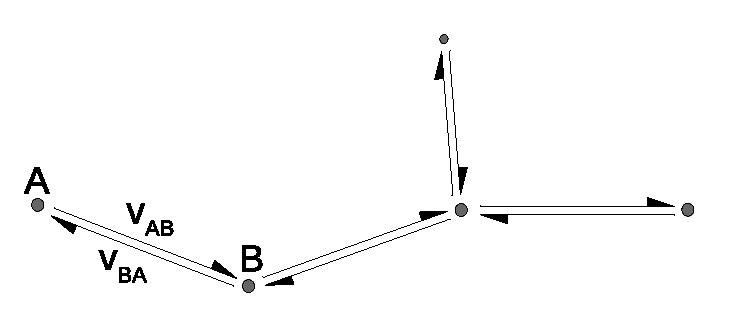
\includegraphics[scale=0.7]{simpleDCELVel}
				\caption{Simple DCEL graph, showing how the edge and velocity from A to B is different from velocity from B to A}
				\label{fig:simpleDCELVel}
			\end{figure}

			In addition to this, not everyone will travel through the mine in the same manner. People who are experienced or impatient might drive faster, while inexperienced or more cautious drivers might drive slower. Speed might also be influenced by time of day, driver's mood, urgency, and a plethora of other reasons. Because of this, the speed over a road segment must be a random variable, a variable with an expected value but that can vary somewhat. The expected value, how much it may vary and the likelihood of such variance is defined by the probability distribution of the random variable. Gaussian distribution, also known as normal distribution, is a commonly occurring distribution, where values close to the mean are common, and values further away from the mean are less so. The probability distribution for the velocity over an edge will be assumed to be Gaussian distributed on the basis that this seems like an intuitive way of driving; Most people following an average speed, with a few driving well above or below that average. Gaussian distributions also have the added benefit of being easy to use mathematically. Denoting velocity as Gaussian distributed is written as

			\begin{equation}
				Velocity \sim N(\mu, \sigma)
			\end{equation}

			$\mu$ denotes the mean, or expected value, of the distribution.

			$\sigma$ denotes the standard deviation, a measure of how wide the spread of possible values is. Variance is a related term which is defined as $\sigma^2$, and more or less explains the same thing. A variable which is not random can be represented with a $\sigma = 0$

			\begin{figure}[H]
				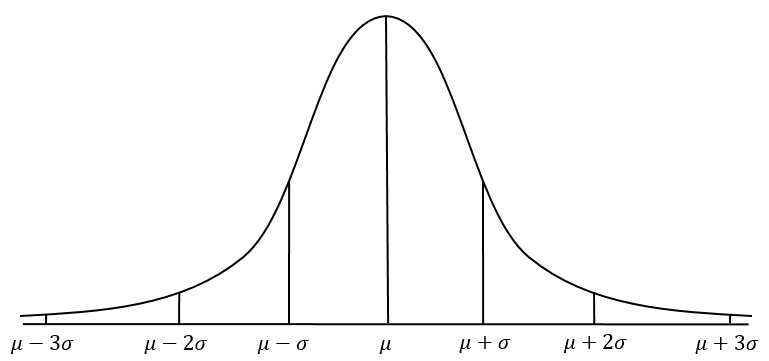
\includegraphics[scale=0.5]{normalDist2}
				\caption{Gaussian distribution. The height denotes how likely a given value is. All Gaussian distributions have the same shape and drop off of probability.}
				\label{fig:normalDist}
			\end{figure}

			The Guassian probability distribution function, as seen in figure \ref{fig:normalDist}, is defined as

			\begin{equation}
				\label{eq:PDF}
				P(x) = \frac{1}{\sqrt{2\pi\sigma^2}}e^{-\frac{(x-\mu)^2}{2\sigma^2}}
			\end{equation}

			Information about random variables, Gaussian distribution and their uses can be found in any statistics maths book, such as \cite{matstat}

			The logs contain historical information about travel in the mine. All logs denoting travel from point A to point B contain a velocity, and all these velocities make up the set of velocities over edge $E_{AB}$. This set of velocities can be used to calculate $V_{AB}$ which is a Gaussian distribution with a mean $\mu$ and a standard deviation $\sigma$. Let $S\{s_1, s_2, ... , s_n\}$ be the set of velocities over $E_{AB}$, the mean $\mu$ for $V_{AB}$ is defined as
			\begin{equation}
				\mu = \frac{s_1 + s_2 + ... + s_n}{n}
			\end{equation}
			As the logs are only a subset of all the travel to ever take place in the mine they are only considered to be a sample. Thus the standard deviation $\sigma$ is a sample standard deviation. It is defined as
			\begin{equation}
				\sigma = \sqrt{\frac{1}{n-1}\sum_{i=1}^{n}(s_i-\mu)^2}
			\end{equation}

			A random variable, such as the velocity, can still be used in normal arithmetic operations. When dealing with only Gaussian distributions addition, subtraction, multiplication, and division are easy and all well defined, and result in a new random variable. However, there is a distinction in arithmetic operations between dependent and independent random variables. In this case, the question of dependence arises in the speed, and subsequently time to cross, of two adjacent edges; if a driver drives quickly/slowly over one edge, will the driver drive equally fast/slow over the next? If the answer is yes then the velocities of adjacent edges are dependent. If the answer is no and the speed across adjacent edges are entirely random then they are independent. Variables can also be somewhat dependent, although taking this into account complicates the mathematics. Exploring absolute dependence and independence give an upper and lower bound. Relevant arithmetic operations are defined below

			\begin{equation*}
				X \sim N(\mu_X, \sigma_X), \mspace{18mu} Y \sim N(\mu_Y, \sigma_Y)
			\end{equation*}
			\begin{equation*}
				X + Y = Z
			\end{equation*}
			\begin{equation*}
				X - Y = Q
			\end{equation*}

			\begin{equation}
				Dependent: Z \sim N(\mu_X + \mu_Y, \sigma_X + \sigma_Y)
			\end{equation}
			\begin{equation}
				Independent: Z \sim N(\mu_X + \mu_Y, \sqrt{\sigma_X^2 + \sigma_Y^2})
			\end{equation}
			\begin{equation}
				Independent: Q \sim N(\mu_X - \mu_Y, \sqrt{\sigma_X^2 + \sigma_Y^2})
			\end{equation}
			No dependent subtraction occurs in this thesis

			Seeing as both distance of an edge and velocity probability distribution over an edge is known it is very natural to get the time probability distribution of crossing an edge by dividing distance with velocity. Unfortunately, dividing by a Gaussian distribution does not result in another Gaussian distribution, but a ratio distribution. This complicates things a lot, and a Gaussian distributed result would be much more preferred. A Gaussian distributed result can be achieved by approximating the division with linearisation instead. Linearisation is done by finding the tangent of the function at the point of $\mu_{distance}$ and $\mu_{velocity}$. Linearisation provides a fairly good approximation close to the tangent intersection, and a poorer approximation further away from this intersection. Thus the lower the variance of the random variable used as the denominator the better the approximation will be, and conversely, the higher the variance the poorer the approximation reflects reality.

			\begin{figure}[H]
				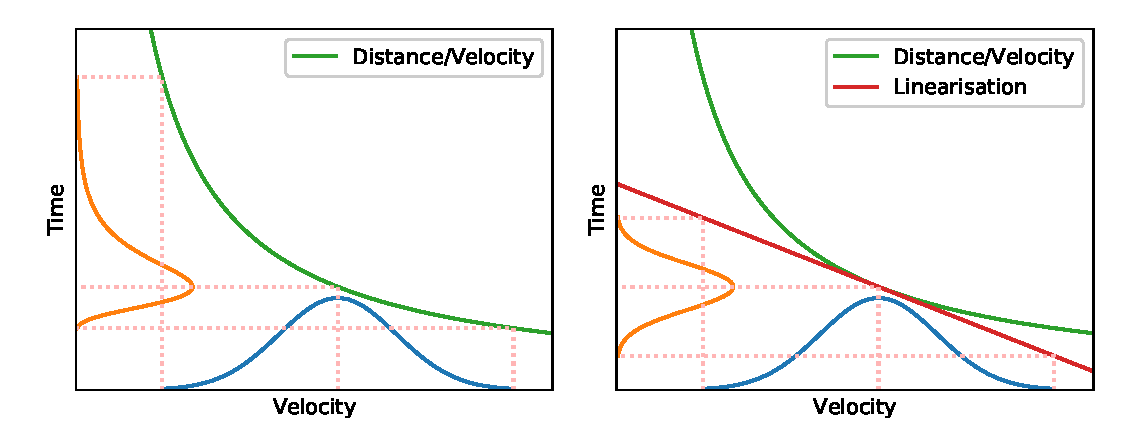
\includegraphics[scale=0.6]{linearisation.eps}
				\caption{Visualisation of linearising division for a constant value of distance.\\ Note that height of curve denotes probability}
				\label{fig:VisualiseLinearisation}
			\end{figure}

			Let $T$ denote time, $D$ distance, and $V$ velocity

			\begin{equation}
				T = f(D,V) = \frac{D}{V} \approx aD + bV + c
				\label{eq:lineraiseT}
			\end{equation}

			\begin{equation}
				a = \frac{d f(\mu_D, \mu_V)}{dD} = \frac{1}{\mu_V}
				\label{eq:linearA}
			\end{equation}

			\begin{equation}
				b = \frac{d f(\mu_D, \mu_V)}{dV} = \frac{-\mu_D}{\mu_V^2}
				\label{eq:linearB}
			\end{equation}

			\begin{equation}
				c = f(\mu_D, \mu_V) - a\mu_D - b\mu_V = \frac{\mu_D}{\mu_V}
				\label{eq:linearC}
			\end{equation}

			The normal notation of division will be kept throughout this thesis, but henceforth refers to linearisation of division.

			With the material discussed in this section a velocity probability distribution can be obtained for every road segment in the mine. These velocity probability distributions can be used to obtain the time probability distribution to cross any given edge, and the resulting time probability distributions can be added together or subtracted.

		\subsection{Basic prediction}
			We consider the most basic example, where two vehicles meet along a straight stretch of road with a few meeting slots to choose from. One vehicle will be defined as having higher priority and will thus not give way. The other vehicle must decide what meeting slot along the road is most appropriate to wait at, and preferably not have a collision while trying to reach that meeting slot.%This problem will be solved using the knowledge of the position for both vehicles, with an associated timestamp and accuracy rating in terms of a standard deviation, and the velocity probability distribution for each segment of road for those types of vehicle.

			\begin{figure}[H]
				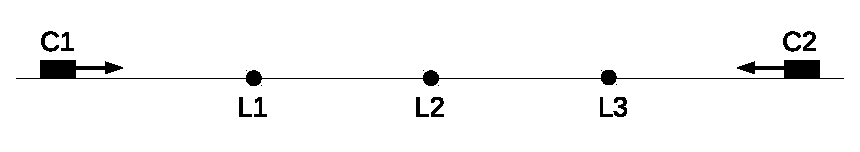
\includegraphics[scale=0.8]{simpleExampleRisksSimple}
				\caption{Basic example. $C_1$ and $C_2$ will collide if no evasive action is taken}
				\label{fig:simpleExampleRisk}
			\end{figure}

			We observe our scenario in Figure \ref{fig:simpleExampleRisk}. $L_1$, $L_2$, and $L_3$ are points at which a vehicle can park in order to let another pass, $C_1$ and $C_2$ are vehicles travelling towards each other. $C_2$ will be given higher priority, and should thus be able to pass through undisturbed, therefore we only focus on the perspective of $C_1$. $C_1$ will have to calculate the risk of attempting to reach $L_1$, $L_2$ and $L_3$, and based on this a decision can be made of where to park.

			The following data is available to solve the problem. X denotes the number of a vehicle. Y denotes the number of a point.

			\begin{tabular}{l l}
			Known variables: & \\
				$dist(A, B)$ & Distance between A and B \\
				$now$ & The current time \\
				$timestamp_{C_X}$ & Timestamp for position for $C_X$ \\
			& \\
			Random variables: &\\
				$LR_{C_X}$ & Reported position for $C_X$\\
				$L_{C_X}$ & Current position for $C_X$ \\
				$\Delta{t}_{L_Y}$ & Difference in vehicle arrival time to $L_Y$\\
				$vel(A, B)$ & Velocity probability distribution from position A to B\\
			\end{tabular}

			For the sake of simplicity it is assumed that all random variables are Gaussian distributed.

			Since positional data might be old $LR_{C_X}$ could represent an old position. To get the current, initial position $L_{C_X}$

			\begin{equation}
				L_{C_X} = LR_{C_X} +  vel(LR_{C_X}, L_{C_X}) \boldsymbol{\cdot} (now - timestamp_{C_X})
			\end{equation}

			It's important to note that the reported position of both vehicles might be old. If the information of one's own vehicle's position is provided from one's own vehicle and not an external source however then $L_{C_X} = LR_{C_X}$ is most probably true!

			What is sought is to calculate is the difference in arrival time, $\Delta{t}_{L_Y}$, from $C_1$'s perspective for all values of $Y$. This will give us a normal distribution of the probability of the difference in arrival times for both vehicles. Negative values are the probability that $C_2$ arrives before $C_1$ and that a collision would take place in attempting this, positive values mean the inverse. Large probability of positive values is therefore desirable.

			To calculate difference in arrival time all that's needed is to add up the time it takes $C_1$ to travel along each road segment leading to $L_Y$, and subtract the time it takes $C_2$ to do the same. Let $S = \{x_1,x_2,...,x_n\}$ denote the set of positions for $C_1$ leading up to a position $L_Y$, and $K = \{y_1,y_2,...,y_m\}$ is the same but $C_2$. The special cases $x_0$ and $y_0$ denotes the initial position of $C_1$ and $C_2$ respectively, which might be unknown and thus a Gaussian distribution.

			To get the time to travel from one location, $A$, to another, $B$, one simply takes the distance between them and divides by the velocity used to travel between the locations.

			\begin{equation}
				t = \frac{dist(A, B)}{vel(A, B)}
				\label{eq:simpleT}
			\end{equation}

			The total time to travel along the set of locations $S$ to the location $L_Y$ for vehicle $C_1$ would be the sum of the times required to travel along each and every road segment leading to $L_Y$

			\begin{equation}
				t_{L_Y} = \sum_{i=1}^{n} \frac{dist(x_{i-1}, x_i)}{vel(x_{i-1}, x_i)}
				\label{eq:sumT}
			\end{equation}

			The difference in time for $C_1$ and $C_2$ to reach a given point $L_Y$ is the difference between the total times it takes for them to travel along their respective sets of points, $S$ and $K$, leading to $L_Y$. It is assumed that the time for two vehicles to reach a point from two opposite directions is independent of each other.

			\begin{equation}
				\Delta{t}_{L_Y} = \sum_{i=1}^{n} \frac{dist(x_{i-1}, x_i)}{vel(x_{i-1}, x_i)} -\sum_{j=1}^{m} \frac{dist(y_{j-1}, y_j)}{vel(y_{j-1}, y_j)}
				\label{eq:deltaT}
			\end{equation}

			The resulting value for $\Delta{t}_{L_Y}$ is a Gaussian distributed variable, with a given $\sigma$ and $\mu$. That which is sought is to find out how likely it is for $C_1$ to reach a point before $C_2$, and thus can attempt to undertake such a traversal. The distribution for $\Delta{t}_{L_Y}$ represents the probability that the vehicles arrive with a given difference in time. A value of zero would mean that both vehicles arrived at the same time. A value less than zero means $C_1$ arrived first by that many seconds, and a value greater than zero means that $C_2$ arrived first by that many seconds. The chance that $C_2$ arrives first is the probability that $\Delta{t}_{L_Y}$ is greater than zero. By integrating over the probability distribution function for a Gaussian distribution (\ref{eq:PDF}) from zero onwards one obtains the probability that $C_1$ arrives at $L_Y$ before $C_2$.

			\begin{equation}
				P(\Delta{t}_{L_Y} \geq 0) = \int_0^\infty \frac{1}{\sqrt{2\pi\sigma^2}}e^{-\frac{(t-\mu)^2}{2\sigma^2}} dt
			\end{equation}

			With $\mu$ and $\sigma$ given from $\Delta{t}_{L_Y}$.

			With these calculations for every point between $C_1$ and $C_2$ an educated decision can be made for what point should be attempted to reach. The point which allows for the most travel and least delay would be chosen. This would be the point furthest from $C_2$, as waiting at an early point would result in a large delay. It is also important to note that the probabilities might be updated as the vehicles traverse. With new positioning information as the vehicles get closer, the algorithm will become more certain of the outcome, which might change its predictions.

			An example of the result values might be
			\begin{equation*}
				\begin{split}
					P(L_1>0)=0.98 \\ P(L_2>0)=0.65 \\ P(L_3>0)=0.22
				\end{split}
			\end{equation*}

			There needs to be a value $R$ which declares what risk a vehicle is ready to accept. If $R$ is $0.6$, then $L_2$ would be an acceptable choice. Consequently, this would result in a higher rate of collision resolutions failing and ending up in a collision. The worst case rate of failure would be $40\%$, although the actual rate would most likely be lower, as not all situations would result in having exactly $60\%$ chance of reaching a point.

			 If $R$ was higher, say $0.8$, then $L_2$ would not be a valid choice, and $L_1$ would be chosen instead. This would result in almost certain success of avoiding a collision, but might also result in a higher overall delay.

			The optimal value for $R$ would depend heavily on the mine in question. It might even be affected by the wishes from management and the drivers themselves. It should, however, be publicly known, so other vehicles can make predictions on what a given vehicle will do. The reason for this becomes apparent in the upcoming sections.

		\subsection{Road clearance}
		\label{sec:RoadClearance}
			Determining road clearance is necessary to resolve more complex problems. For two vehicles on collision course determining clearance is quite straight forward. As in the simple example visualized in Figure \ref{fig:simpleExampleRisk}, determine if the vehicles are going to collide and find a meeting slot to park in order to prevent this. The most basic example where clearance fails is when two vehicles on a collision course are travelling along the same road segment with no meeting slots in between them. In such a situation a collision is unavoidable which is highly undesirable. This is avoidable by solving the collision before there comes a point where no meeting slots exist between the two vehicles.

			A less obvious example might be when two vehicles travel together in the same direction. Since they travel in the same direction they will not collide and can travel close together. Two or more vehicles travelling together in the same direction will be referred to as a caravan. If a caravan of two vehicles find a collision course with an oncoming vehicle with higher priority and attempt to solve the collision naively clearance will fail. The first vehicle will occupy the most optimal meeting slot, the one closest to where the collision would take place, leaving the second vehicle without any meeting slot to park at and thus be on an unavoidable collision course. It is therefore apparent that vehicles must take into account the vehicles around them, and their solutions to collisions they experience. This applies also when the cars are not directly linked in a caravan.

			\begin{figure}[H]
				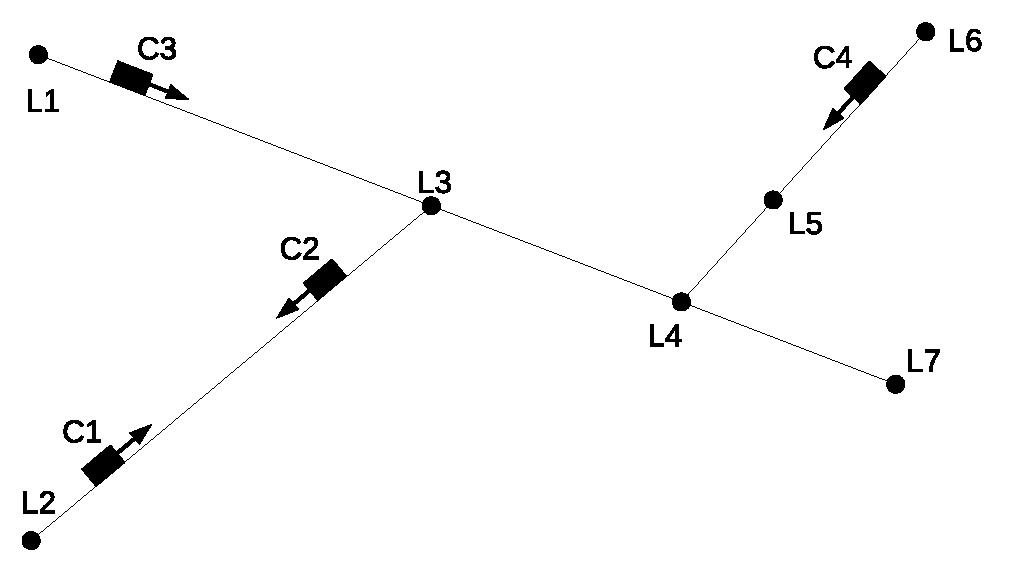
\includegraphics[scale=0.5]{advancedClearanceHori.eps}
				\caption{More complicated scenario highlighting determining clearance}
				\label{fig:advancedClearance}
			\end{figure}

			Study the scenario in Figure \ref{fig:advancedClearance}. The priority of every vehicle is assigned the same as their numbering, i.e. $C_1$ has the highest priority, $C_2$ next highest, etc. At $L_5$ there exists a meeting slot to park in. $L_3$ and $L_4$ are junctions which can also be used to give way at but that do not have meeting slots. The vehicles have the following destinations

			\begin{tabular}{l l l}
				$C_1$ & $\rightarrow$ & $L_7$ \\
				$C_2$ & $\rightarrow$ & $L_2$ \\
				$C_3$ & $\rightarrow$ & $L_6$ \\
				$C_4$ & $\rightarrow$ & $L_7$ \\
			\end{tabular}

			First off, $C_1$ has the highest priority. This vehicle will not have to make way for anyone. Directly in the path of $C_1$, however, lies $C_2$, who needs to make way. There are no places to park between $C_1$ and $C_2$, so $C_2$ will need to back up immediately. The most optimal way for $C_2$ to make way is to park in the road segment $L_3L_1$, thus blocking $C_3$ until $C_1$ passes. If $C_3$ was not blocked, it would reach $L_4$ before $C_4$ would have. Thus if $C_4$ simply takes into consideration the predicted travel of $C_3$, and not that of $C_1$ or $C_2$, it would decide that it needs to park and wait in the meeting slot at $L_5$ for $C_3$ to pass. If so consider the case if more vehicles with the same priority and route as $C_1$ appear in short intervals, leaving $C_2$ and $C_3$ locked, and $C_4$ waiting for a collision that will never happen. In such a scenario $C_4$ is affected by a vehicle, $C_2$, that in no way intersects with its own path.

			Another example is if $C_3$ has the same priority as $C_1$ and may absolutely not stop, and also shares the destination of $L_7$. In such a scenario $C_2$ might find itself being pushed in front of the two vehicles $C_1$ and $C_3$ until it reaches the road segment $L_4L_6$, in which case $C_4$ will encounter an interrupt from a vehicle it does not share a path with.

			It becomes apparent that the formula for calculating the time difference for two vehicles arriving at a given point must also include the delays for both vehicles incurred while en route to the given point. This delay is also a random variable, being constructed from the parameters of the third party vehicles causing the delay. Letting $D(C_X, A)$ denote the delay vehicle $C_X$ experiences at position $A$ and Equation \ref{eq:deltaT} can be expanded. $C_{self}$ is the vehicle doing the calculations and $C_{other}$ is a vehicle it might collide with.

			\begin{equation}
				\Delta{t}_{L_Y} = \sum_{i=1}^{n} \bigg(\frac{dist(x_{i-1}, x_i)}{vel(x_{i-1}, x_i)} + D(C_{self}, x_i)\bigg) -\sum_{j=1}^{m} \bigg(\frac{dist(y_{j-1}, y_j)}{vel(y_{j-1}, y_j)} + D(C_{other}, y_i)\bigg)
				\label{eq:deltaTdelay}
			\end{equation}
			%(should the delay be for $i$ and not $i-1$?)

		\subsection{Delays}
		\label{sec:Delays}

		As uncertainties are at play, it is not always a certainty that a delay will be incurred. Because of this, there might be diverging branches of possibilities arising from this. One for where a delay was incurred, and one for where it did not. Both possibilities will be represented by their own normal distribution for that particular branch. Such an occurrence can be modelled using a Gaussian mixture model, GMM. A GMM combines several component Gaussian distributions, i.e. normal distributions, into one singular model. Every component has a weight, and the sum weight of all components adds up to 1, representing the total probability of events. Thus if there is a 30\% chance of incurring a delay that branch of events and subsequent distribution would be given a weight of 0.3, and integrating the area under this component only would give a value of 0.3. The opposite branch is subsequently given a weight of 0.7.

			\begin{figure}[H]
				\includesvg[scale=0.6]{GMM}
				\caption{An example from the web \cite{GMMImage} of a three component GMM with seemingly equal weight for each component. Dashed line shows the components, full line shows distribution.}
				\label{fig:GMM}
			\end{figure}

			For a univariate case, as is the case in this scenario, the mixture model is described as the sum of the K component distributions, where K can be any positive integer. $\phi$ denotes the weight.

			\begin{align}
				p(x) &= \sum_{i=1}^K\phi_i \mathcal{N}(x \;|\; \mu_i, \sigma_i)\\
				\mathcal{N}(x \;|\; \mu_i, \sigma_i) &= \frac{1}{\sigma_i\sqrt{2\pi}}e^{-\frac{(x-\mu_i)^2}{2\sigma_i^2}}\\
			\end{align}

			A delay will be incurred every time two vehicles meet since one vehicle needs to park to let the other pass. Parking early would result in a bigger delay than parking later, and which is incurred is uncertain. Consider the following scenarios

			\begin{figure}[H]
				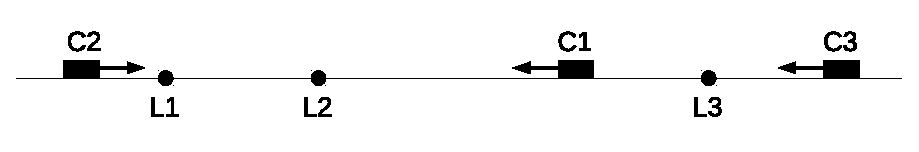
\includegraphics[scale=0.8]{delayProbability.eps}
				\caption{Scenario depicting delay uncertainty about $C_2$ from the perspective of $C_3$}
				\label{fig:delayProbability}
			\end{figure}

			In figure \ref{fig:delayProbability} priority is assigned in the same order as the numbering. $C_1$ highest, $C_3$ lowest. $C_1$ does not have to care about anything and should simply drive. $C_2$ cares only about where it will meet $C_1$, and whether it should park at $L_1$ or $L_2$ to give way. $C_2$ has a probability for reaching both of them ahead of $C_1$. Assuming that $C_2$ has a $70\%$ chance to reach $L_2$ before $C_1$ does, and goes with this option, there's a $30\%$ chance that it will not. In the case of $C_2$ reaching $L_2$ first the delay $C_2$ incurs will be the same as the time needed for $C_1$ to reach $L_2$, which is already defined in $\Delta{t_{L_2}}$ for $C_2$. In the case of $C_2$ not reaching $L_2$ before $C_1$, then $C_2$ needs to reverse back to $L_1$. A lot of factors may contribute to the delay in such a scenario. For instance how much heads up $C_2$ is given before needing to reverse, and maybe $C_1$ needs to slow down as it waits for $C_2$ to reverse. Reversing speed is however not a variable readily available for this thesis. The delay incurred at $L_1$ is either the time needed by $C_2$ to reverse to $L_1$ or the time required for $C_1$ to reach $L_1$, whichever is greater.

			$C_3$ does not know which delay $C_2$ will suffer, however, it can estimate the probability. Both the scenarios of where $C_2$ has to park are important to consider as their distributions might overlap when $C_3$ estimates its chances to reach any given point.

			To summarize section \ref{sec:RoadClearance} and \ref{sec:Delays}, vehicles must consider the actions and decisions made by vehicles in their surrounding. Easily one can consider doing this recursively as soon as a vehicle intersects with another's path.

		\subsection{Search space}
			The idea behind heuristics is that one need not compute the entire system to its end to obtain a result. The question is then how far along its own path a vehicle should estimate chances for collisions. In the most basic case, a vehicle must only make sure that it has at least one meeting slot free to park in to make sure it can give way in case of a collision. As such it only needs to explore the space ahead enough to make sure that no other vehicle could beat it to that meeting slot. The distance of exploration is closely tied to the time of travel for vehicles. The upper bound of the exploration would be defined by the furthest distance away the fastest vehicle could be while travelling at the fastest probable speed and make it to the meeting slot first if the exploring vehicle travels the slowest probable speed. Probable speed will be defined as within two standard deviations of the estimated speed. For a Gaussian distributed random variable to take a value outside of two standard deviations from the mean has a chance of 2.257\% \cite{matstat}. Thus there is a 2.275\% chance that a vehicle travels slower than the slowest probable speed, and an equal chance it travels faster than fastest probable speed. For both events to occur simultaneously would have a probability of

			\begin{equation}
				0.02275 \boldsymbol{\cdot} 0.02275 = 0.0005175625
			\end{equation}

			so a 0.05\% risk.

			With this methodology, if the exploring vehicle is 200m away from the closest meeting slot, and its slowest probable time to arrive there is 40 seconds, the exploration space would be however far the fastest vehicle in a probable manner could travel in 40 seconds. If the highest probable speed on the other side of the meeting slot is 30km/h, which translates to 8.33 m/s, then the exploration space would be.

			\begin{equation}
				  8.33 \boldsymbol{\cdot} 40 = 333.33m
  			\end{equation}

			That is 333.33m ahead of the meeting slot in question.

			Defining the time it takes the exploring vehicle to reach the meeting slot as $t$ and the highest probable velocity of an approaching vehicle as $h$

			\begin{align}
				t &= \frac{dist(vehicle, meeting slot)}{vel(vehicle, meeting slot)} \\
				h &= vel(meeting slot, onwards)
			\end{align}

			we define the entire equation as

			\begin{equation}
				explore = (\mu_t - 2\sigma_t) (\mu_h + 2\sigma_h)
			\end{equation}

			Before a vehicle passes a meeting slot it must have explored for the next upcoming meeting slot and estimated any potential collisions. In essence, a risk for disregarding the closest meeting slot and going for the next one is what is obtained.

			If an approaching vehicle is found in the exploring area, or any vehicle at all in between the current position and the meeting slot being explored for, the algorithm must be run as if from the eyes of this detected vehicle if this vehicle has higher priority. By running the algorithm from the perspective of the detected vehicle the exploring vehicle can predict what this vehicle will do. This, in turn, can result in finding a third vehicle which is considered. Since every vehicle has a unique priority any cyclic relationships will be nullified by a high priority vehicle simply not caring what a low priority vehicle does, as the low priority vehicle must give way to a high priority vehicle. Consequently, this means that the vehicle with the very lowest priority might find itself recursively iterating through every other vehicle in the mine in the worst case. This is not very useful however, as every step along the way adds a lot of uncertainty. In addition, with lacking connectivity the data possessed by one vehicle might differ from the data held by another and will thus come to different conclusions, further degrading reliability.

    \section{Analysis}
		With the collection of historical traversal data, the predictive model stated in this thesis can be evaluated. This section will do just that.

		\subsection{Velocity data}
			The test data available to this master's thesis is the logs from a number of trucks operating in a mine. The trucks are equipped with the Hybrid Positioning system. The logs contain a lot of information, but the fields relevant to this thesis are that of estimated position in terms of X, Y, and Z axis from the positioning system, a timestamp as well as speed from OBD data. The log entries depict the state of the vehicle at that particular timestamp.

			\subsubsection{Processing logs}
%				{\bfseries Maybe be it's own section??}
				By processing a collection of travel logs a histogram, and consequently a distribution, for the road segments can be found. Suppose we have two log entries for a vehicle.
				\begin{itemize}
					\item Log 1: Coordinates of node A. Speed $15 km/h$
					\item Log 2: Coordinates of node B. Speed $18 km/h$
				\end{itemize}

				From this we can conclude that the vehicle travelled from node A to node B. If node A and node B are neighbours then there will exist an edge $E_{AB}$ that connects them. Thus when processing these logs the edge $E_{AB}$ will have an entry added to it noting that a vehicle travelled across this edge with the speed of $18 km/h$. If a third log directly after Log 2 records the location of node C and a speed of $20 km/h$, and node B and C are neighbours, then the edge $E_{BC}$ between B and C will have an entry added noting that a vehicle travelled across it with the speed of $20 km/h$. By repeating this process for all the thousands of logs, a histogram can be created for those edges which appeared in the logs numerous times.

			\subsubsection{Processing edge cases and problems}

				The logs are not always perfect, so these following edge cases and problems needed to be dealt with

				If two sequential logs point to nodes A and C that are not neighbours, a breadth-first search will be conducted to find the path from A to C. If the path A, B, C is found, then the edges $E_{AB}$ and $E_{BC}$ will both have the speed value of the second log, pointing to C, added to them. The positioning algorithm updates once per second, and since the nodes are spaced out by five meters it is not uncommon for vehicles to travel fast enough to skip nodes in normal operations. $5m/s$ is equivalent to $18km/h$.

				If two sequential logs point to the same node, the later log is simply ignored.

				If two sequential logs 1 and 2 points to two unique nodes that have a Euclidean distance larger than 16 meters then this specific traversal will be ignored. The update frequency for the algorithm is once per second, and to travel 16 meters in one second translates to $57.6km/h$. The speed limit of the mine is $30km/h$, so it is assumed that the positioning algorithm is struggling to pinpoint a position and is making large jumps once it regains accuracy. The processing will resume as normal after the jump.

				The positioning cannot be assumed to be perfect. Sometimes it makes small or large jumps, and sometimes it even staggers backward on itself. However the accurate logs are deemed to heavily outweigh the inaccurate ones and, over the course of thousands of logs, the inaccuracies will simply become noise in the data.

			\subsubsection{Distribution analysis}

				Processing the logs of only vehicles labelled as trucks in the mine between the dates of 2019-03-22 until 2019-05-15 renders 8627641 data points over 16433 nodes and 32956 edges. Every added speed record counts as a data point, even in the case where a node is skipped and the same speed is added to more than one edge. Naturally, some edges are traversed often while some are barely traversed at all, and so edges can have greatly varying amounts of data.

				The original theory stipulated that the histograms of the speed data over these road segments would form a Gaussian distribution. The results confirm this to a degree but also shows the flaw of this assumption. A subsection of the histograms conform very well to a Gaussian distribution, as can be seen in figure \ref{fig:logResGood}.
				\begin{figure}[H]
					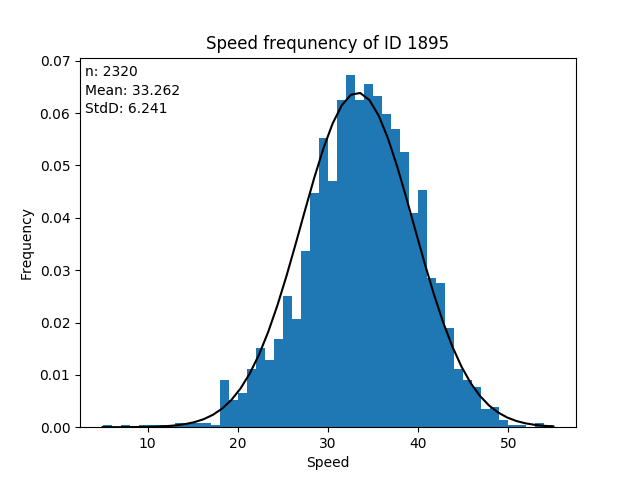
\includegraphics[scale=0.5]{logResGood.png}
					\caption{Normalized histogram of speed over an edge. Gaussian PDF of the set overlaid.}
					\label{fig:logResGood}
				\end{figure}

				Other histograms have poorer fits to a Gaussian distribution, as can be seen in figure \ref{fig:logResEh1} and \ref{fig:logResEh2}.

				\begin{figure}[H]
					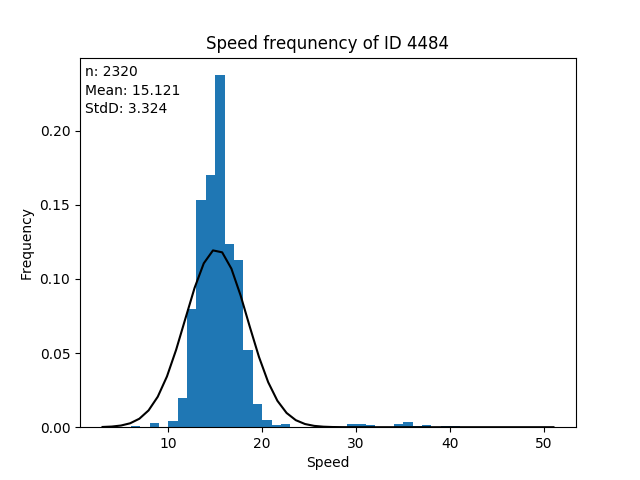
\includegraphics[scale=0.5]{logResEh1.png}
					\caption{Normalized histogram of speed over an edge. Gaussian PDF of the set overlaid.}
					\label{fig:logResEh1}
				\end{figure}

				\begin{figure}[H]
					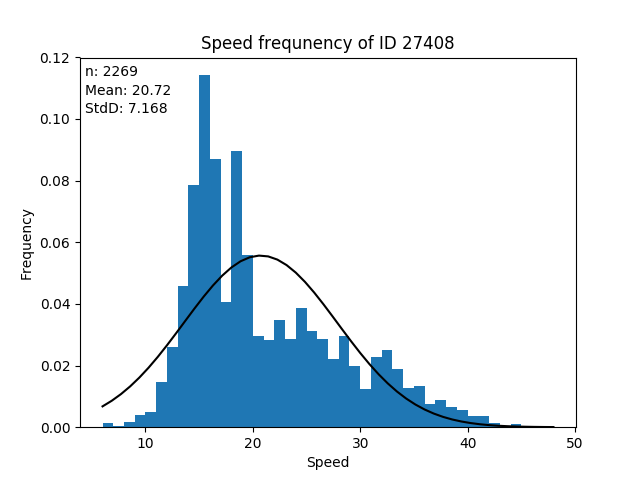
\includegraphics[scale=0.5]{logResEh2.png}
					\caption{Normalized histogram of speed over an edge. Gaussian PDF of the set overlaid.}
					\label{fig:logResEh2}
				\end{figure}

				Another subset of histograms show quite clearly two distinct distributions in the same histogram, as can be seen in figure \ref{fig:logResBad}. One theory is that they represent when the truck is loaded and not loaded respectively, which could have a major impact on traversal speed and behaviour. Another is that these are edges adjacent to a road junction, where vehicles making sharp turns will be travelling slower than those who drive straight through the junction. This shape appears for both when observing only a single truck or collections of several trucks, and is thus not caused by differences in vehicle or driver.

				\begin{figure}[H]
					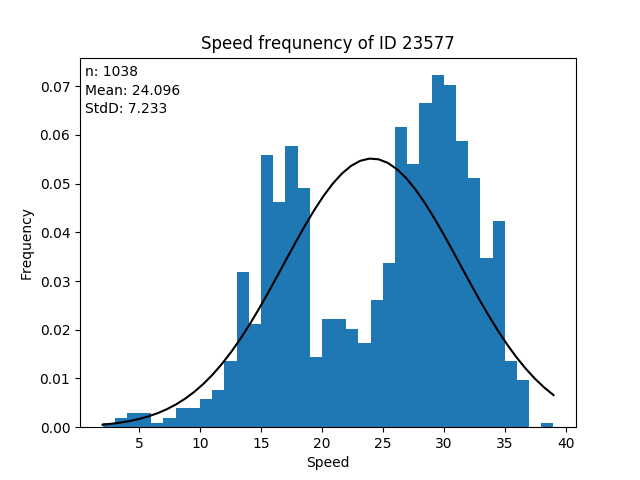
\includegraphics[scale=0.5]{logResBad.png}
					\caption{Normalized histogram of speed over an edge. Gaussian PDF of the set overlaid.}
					\label{fig:logResBad}
				\end{figure}

		\subsection{Testing against real data}
			The logs available to this thesis are somewhat limited in the information they contain. They contain no information regarding loss of connection, meeting other vehicles, or collisions. Neither are these logs correlated to the logs of any other positioning system, either better or worse. This means that with the current set of logs it is difficult to prove anything definitively in terms of dealing with inaccurate positions, loss of connection, or the efficacy of the algorithm in avoiding collisions and improving flow. The logs can, however, prove the efficacy of the predicted difference in arrival time to a point, which can give an indication of how well it would do in preventing collisions in real life scenarios. The efficacy of the predicted difference in arrival time to a point is what will be explored in this section.

			Every edge has a Gaussian distribution of historical traversal velocity calculated as described in the previous section. Using these a prediction of arrival time from a node $A$ to a node $B$ can be calculated, as defined in equation \ref{eq:sumT}. To validate how correct the results of the predictions are they must be compared against actual values pulled from the logs. The relevant set of logs are those that at some point visit point $A$, and then travel to point $B$ through a specified path without diverging. The values obtained from the set of logs between $A$ and $B$ also constitute a set. This set might not necessarily be of a Gaussian distribution. Common values in these results are

			\paragraph{Log Time}
				The difference in time in seconds logged at point $A$ and point $B$.
			\paragraph{Log Speed}
				For every edge along the path between $A$ and $B$, the distance of the edge is divided by the logged speed and added together to obtain total time taken to traverse the path.
			\paragraph{Theory}
				The theoretical prediction of traversal time, as described in this thesis. Can be calculated assuming adjacent edges' velocity distributions are either dependent or independent.

			It is important to note that Log Speed is a subset of the data that Theory is based upon, which in contrast has not been assumed to be Gaussian distributed nor linearised in division. The best that theory can accomplish is thus to mimic Log Speed. Log Time is the value which actually reflects real life though.

			The massive size and complexity of a mine create an innumerable amount of possible points and path combinations. It is therefore impractical to test against every such permutation. Therefore the results displayed will be samples picked in an attempt to show the best, the worst, and average cases. The concept of "how well does this histogram and this distribution fit?" is also very hard to put a number to. Because of this the results and their fit will be analysed mostly visually.

			\subsubsection{Linearisation, dependence and Gaussian assumption}
			\label{sec:dependenceResults}
				Some important questions to answer is how much the assumption of Gaussian distribution and linearisation distorts the result, and how the assumption of dependence or independence of velocity over adjacent edges affect results. To get an idea of this a path is analysed with Log Speed, Theory, and with the addition of a theory which has not been linearised. This non-linearised theory is achieved by generating a normal distributed set of values for each edge from that edge's velocity probability distribution. The distance of the edge is then divided by the values of this set without linearisation, and so result in a set of arrival times which have not been linearised in division. This is done both with the assumption of total dependence and total independence of velocities.

				For shorter distances, such as in the presented result paths covering 10 edges which corresponds to about 45 meters, it is mostly a toss up if dependent or independent variants of the theory fits better. In the case of dependent velocities having a better fit the non-linearised theory has a clear better fit than linearised theory. The histograms of Log Speed sometimes fit a non-linearised Gaussian distribution quite well, and sometimes very poorly.

				\begin{figure}[H]
					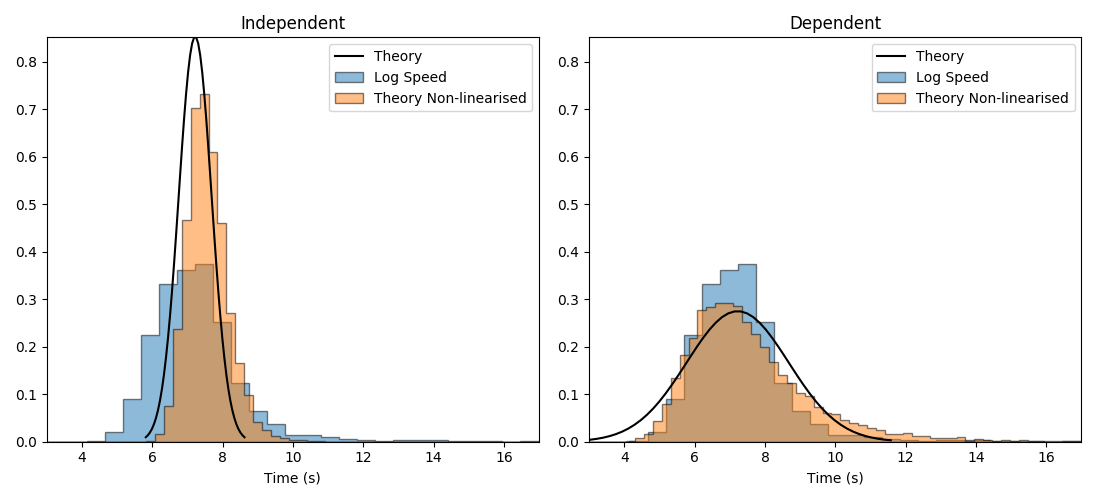
\includegraphics[scale=0.5]{non-lin10-10A.png}
					\caption{Dependent and Independent predictions over a path 10 edges long\\A good fit for dependent velocities}
					\label{fig:non-linShort1}
				\end{figure}
				\begin{figure}[H]
					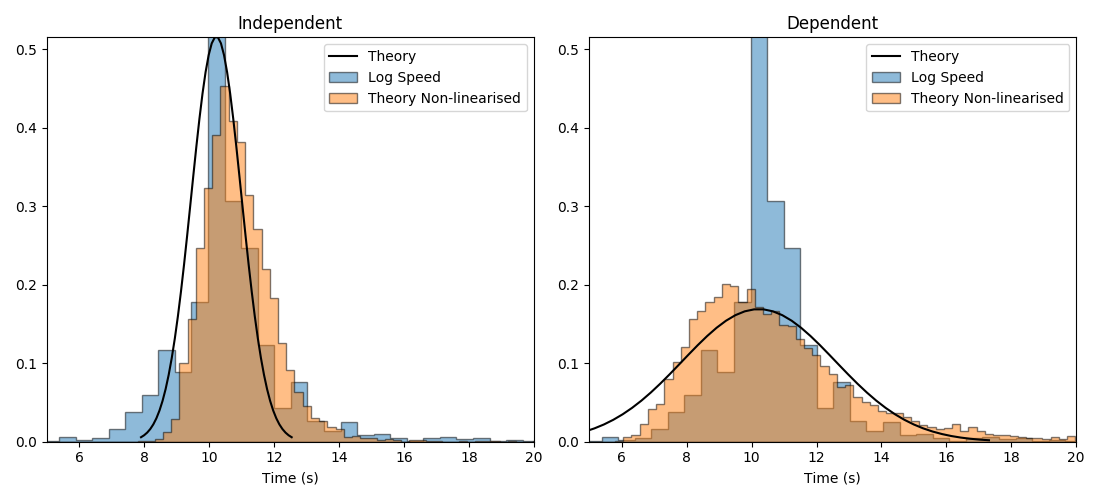
\includegraphics[scale=0.5]{non-lin10-10B.png}
					\caption{Dependent and Independent predictions over a path 10 edges long\\A better independent fit}
					\label{fig:non-linShort2}
				\end{figure}
				\begin{figure}[H]
					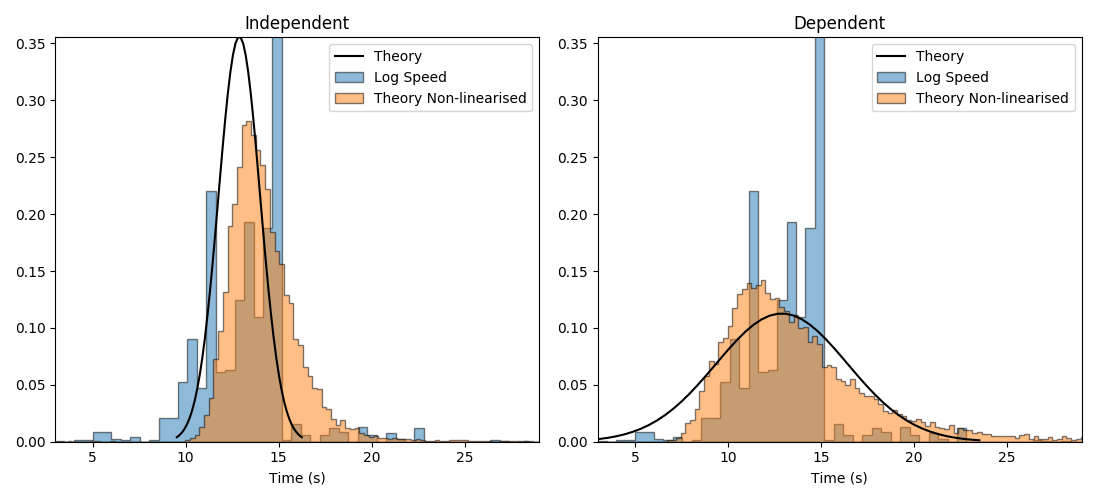
\includegraphics[scale=0.5]{non-lin8-10A.png}
					\caption{Dependent and Independent predictions over a path 10 edges long\\Not a great fit for either, and not a good fit for Gaussian distribution}
					\label{fig:non-linShort3}
				\end{figure}

				Over longer distances it becomes apparent that dependent velocities create a much better fit overall, even on those paths where independent velocities had a better fit at shorter distances. The fits are not always perfect, however, and the Gaussian properties of Log Speed are sometimes great, sometimes not.

				\begin{figure}[H]
					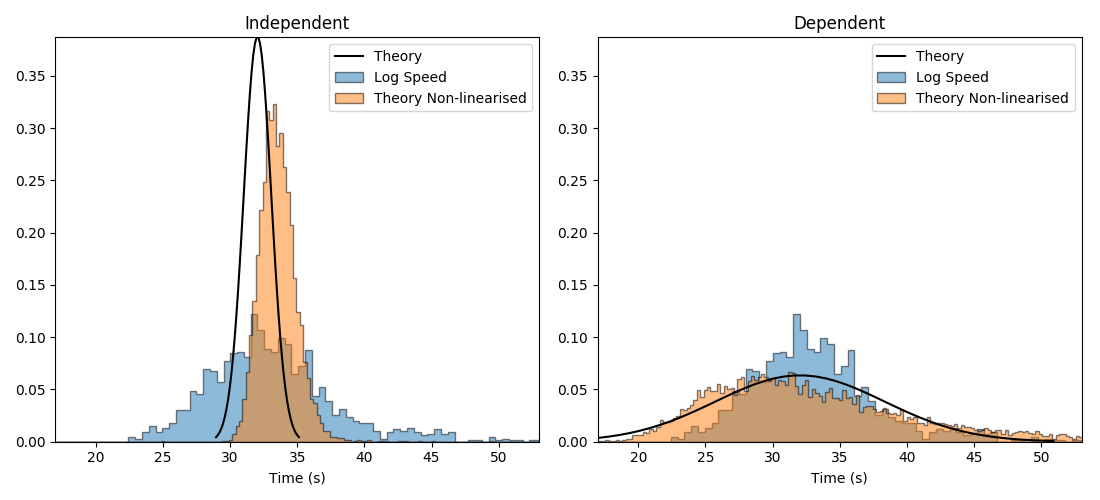
\includegraphics[scale=0.5]{non-lin10-40B.png}
					\caption{Path ending in same node as figure \ref{fig:non-linShort2}, but now 40 edges long}
					\label{fig:non-linLong1}
				\end{figure}
				\begin{figure}[H]
					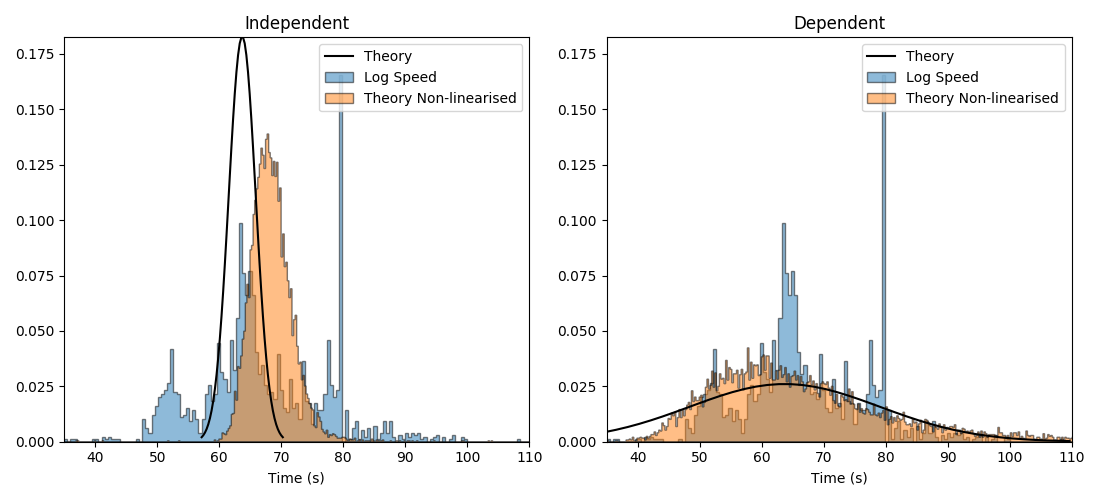
\includegraphics[scale=0.5]{non-lin8-50A.png}
					\caption{Path ending in same node as figure \ref{fig:non-linShort3}, but now 50 edges long\\Not great Gaussian fit}
					\label{fig:non-linLong2}
				\end{figure}
				\begin{figure}[H]
					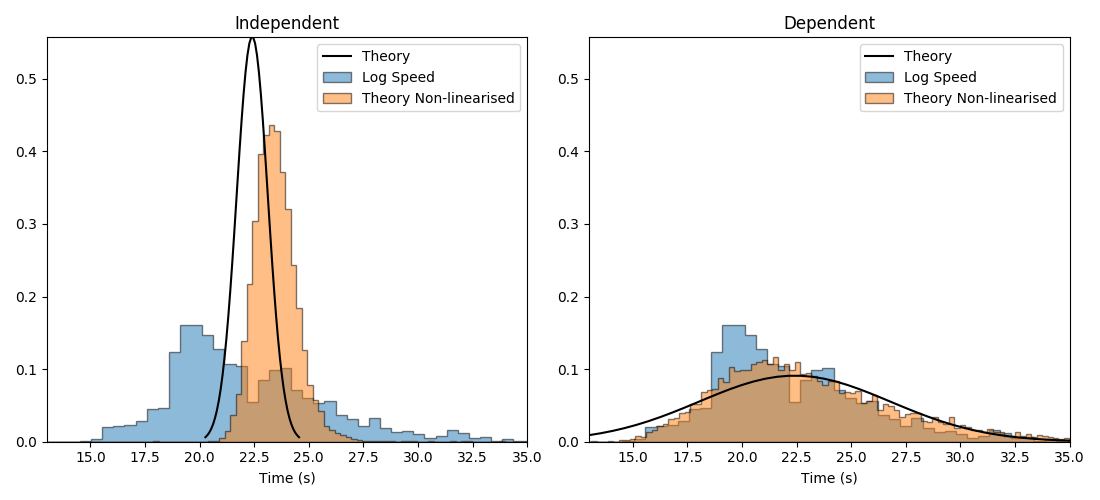
\includegraphics[scale=0.5]{non-lin12-40A.png}
					\caption{40 edges long path. Log Speed follows expected shape of Gaussian non-linearised division}
					\label{fig:non-linLong3}
				\end{figure}

			\subsubsection{Predicting differnece in arrival}

				To predict the difference in arrival time the values for two paths which both ends in the same point are subtracted. This is defined in the theory in equation \ref{eq:deltaT}. These results contain no non-linearised results but are instead meant to showcase the accuracy of the solution algorithm at hand. Theory is presented with both independent and dependent addition.

				\begin{figure}[H]
					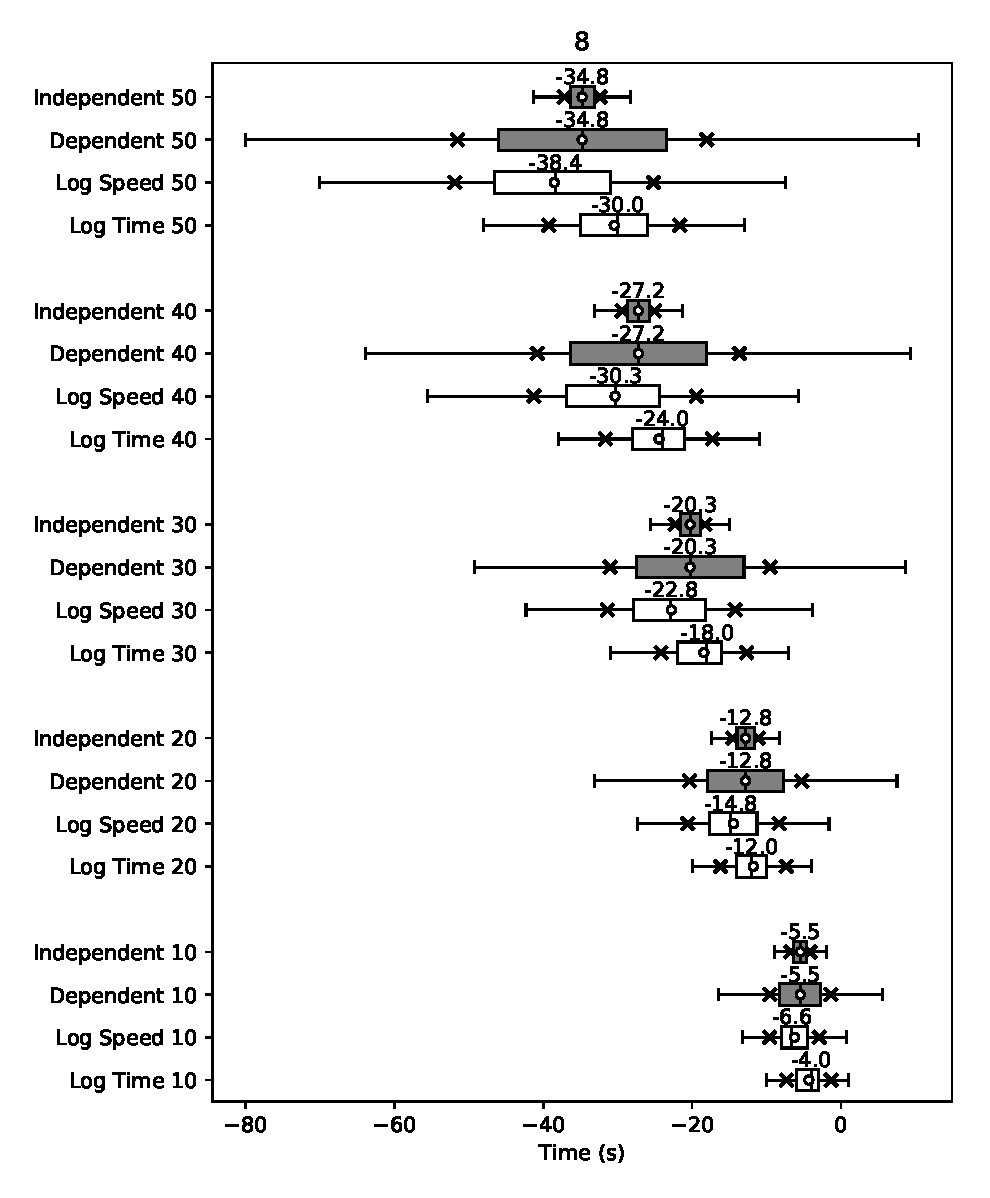
\includegraphics[scale=0.7]{8.eps}
					\caption{Result of prediction and actual log times to a node. Mean represented by a line and written out, median by a circle, and X denotes standard deviation}
					\label{fig:box1}
				\end{figure}
				\begin{figure}[H]
					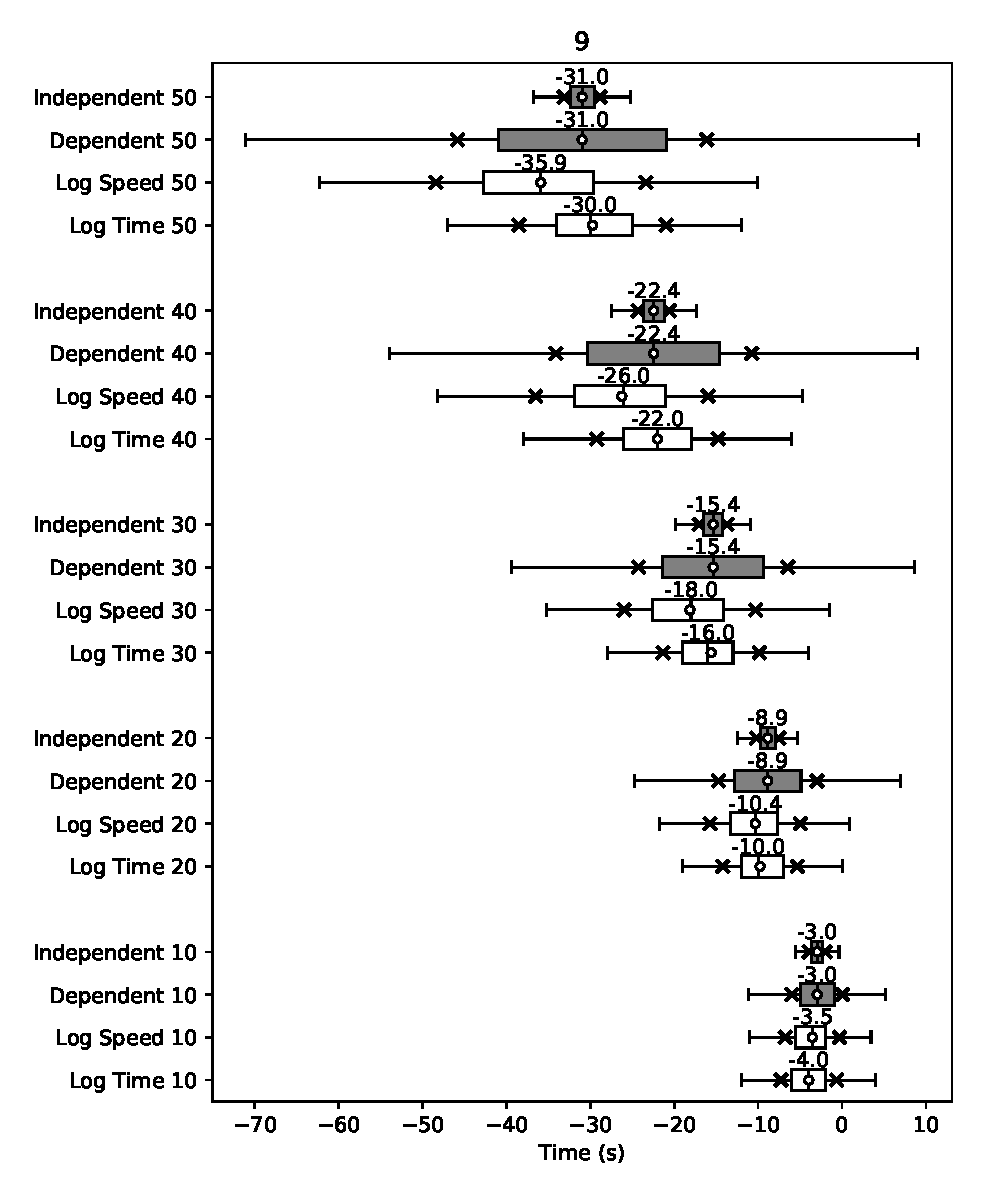
\includegraphics[scale=0.7]{9.eps}
					\caption{Prediction and actual log times to a node. Mean represented by a line and written out, median by a circle, and X denotes standard deviation}
					\label{fig:box2}
				\end{figure}
				\begin{figure}[H]
					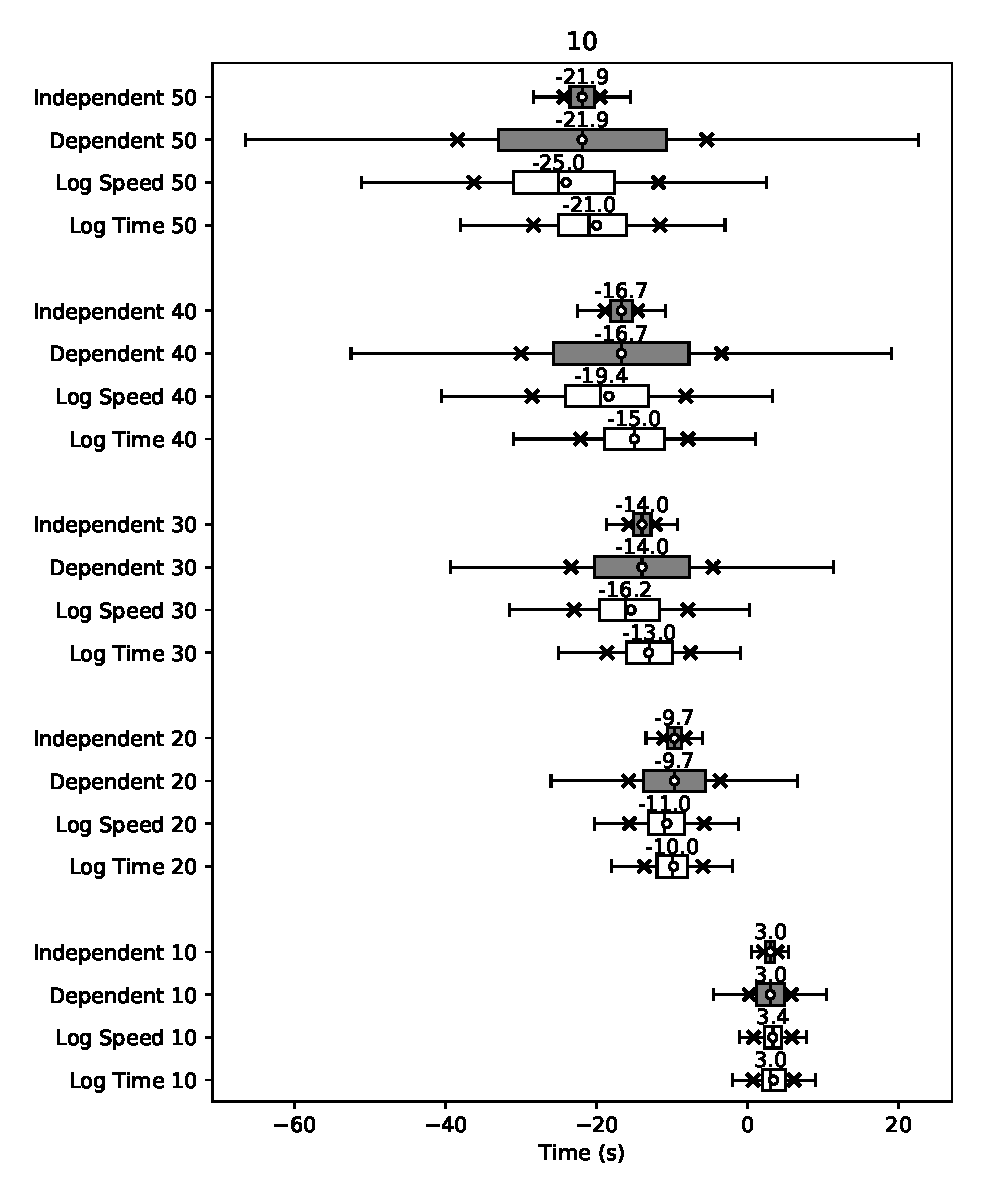
\includegraphics[scale=0.7]{10.eps}
					\caption{Prediction and actual log times to a node. Mean represented by a line and written out, median by a circle, and X denotes standard deviation}
					\label{fig:box3}
				\end{figure}

				In these results, the actual value in seconds obtained matters little. All that matters is that the prediction mimics the actual results observed. It is obvious that the values predicted by the algorithm follow the mean of the actual values quite closely, but the variance of the independent prediction is much too small, and the variance of the dependent prediction seems to be slightly too large. This seems to be a trend throughout all the data points observed.

			\subsubsection{Old data}
				A set of older logs exist, containing 1694909 data points between the dates of 2019-01-31 until 2019-03-18. These are used to create velocity probability distributions and then comparing the predictions made by this old data against newer logs. This way an analysis can be done of the validity of the data over time. The results show a very slight difference, but not very significant. In most cases, the difference actually moves the predicted mean closer to that of the actual logs.

				\begin{figure}[H]
					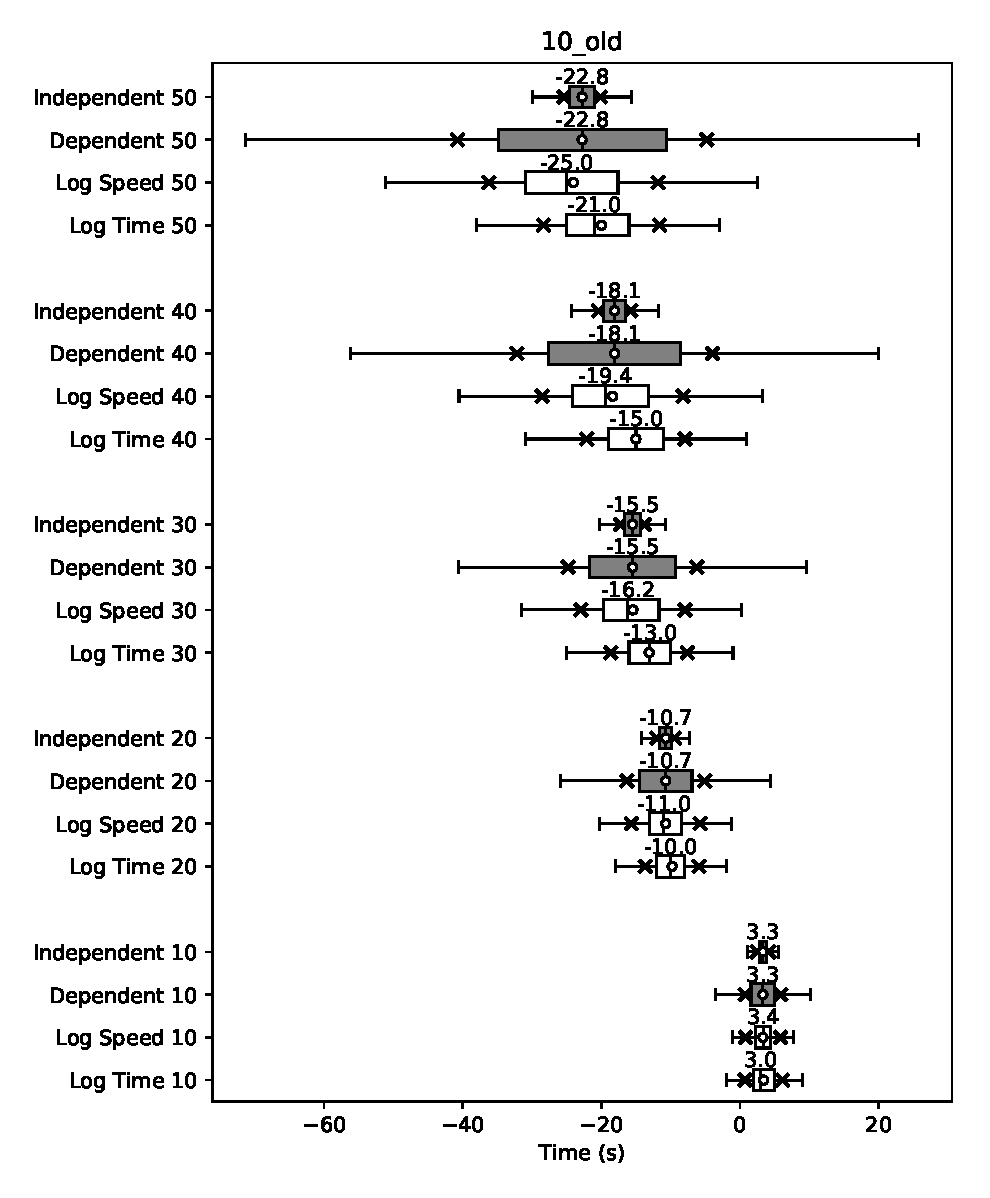
\includegraphics[scale=0.7]{10_old.eps}
					\caption{Prediction using old data and new logs, same mid point as figure \ref{fig:box3}}
					\label{fig:oldWithNew}
				\end{figure}


			\subsubsection{Low amounts of data}
				%Can't run tests on places with few logs. How about make artificially low data structure by taking a subset for DCEL, and test in common places
				A lot of edges contain very little data, such as containing less than 100 data points. At these levels, the statistical models can be very vulnerable to singular outliers.

				Testing how these low data places hold up in prediction is hard, as there are very few logs to test against. So to test the predictions for low amounts of data a place with high amounts of data is chosen, the velocity distributions are built up using a very small subset of all data and then tested against the full set of logs. The predictions made using low amounts of data seems to consistently have a higher variance those made with more data.

				\begin{figure}[H]
					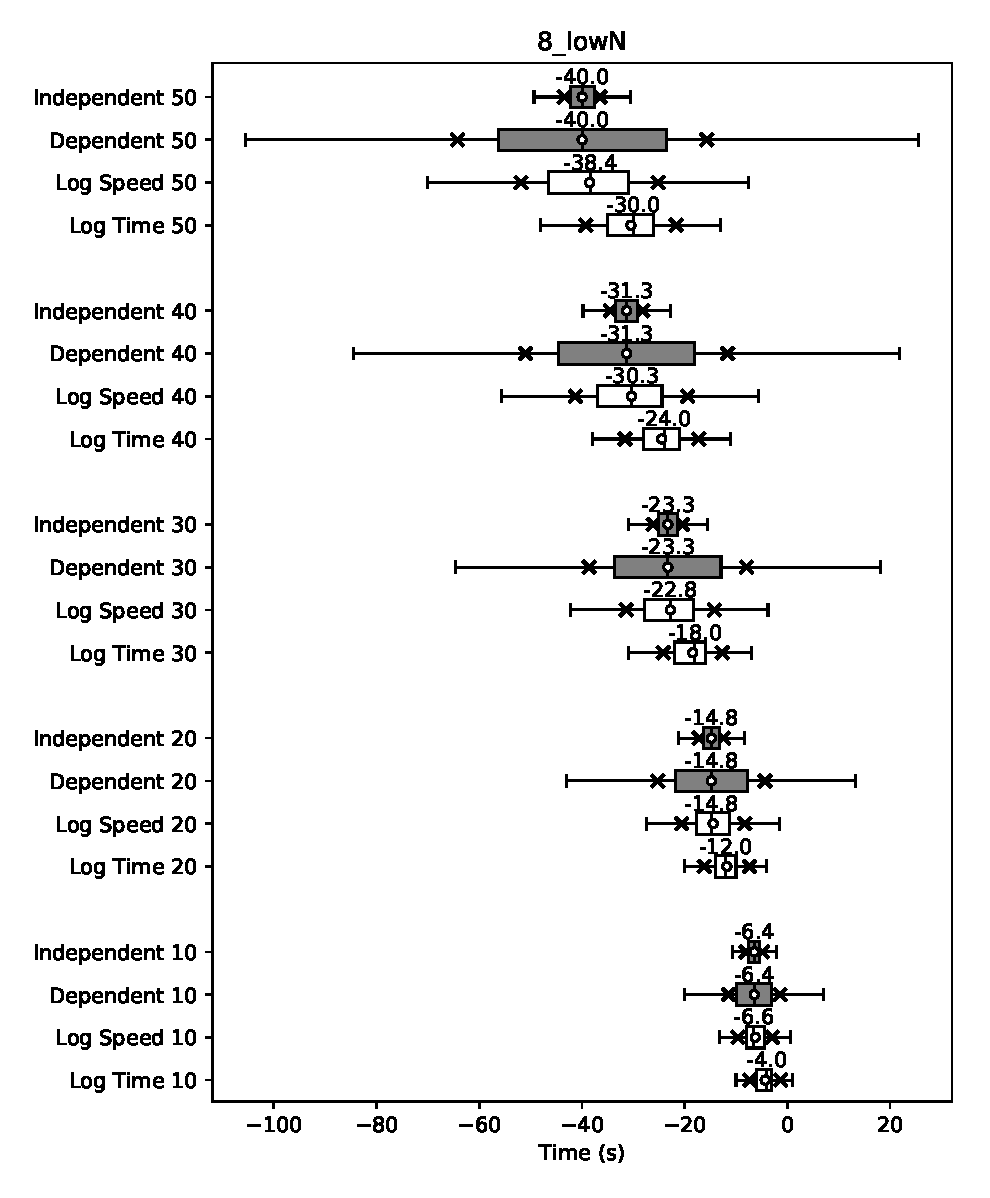
\includegraphics[scale=0.7]{8_lowN.eps}
					\caption{Same node as figure \ref{fig:box1}. Velocity probability distribution for edges in the paths are made with around 40 to 50 data points.}
					\label{fig:lowN1}
				\end{figure}

			\subsubsection{Cross referencing}
				It could be a concern that the predictions of travel are compared against the same logs from which the statistical models were created. Therefore a quarter of the logs were separated and test run again for these. The results show no significant change from previous results.

				\begin{figure}[H]
					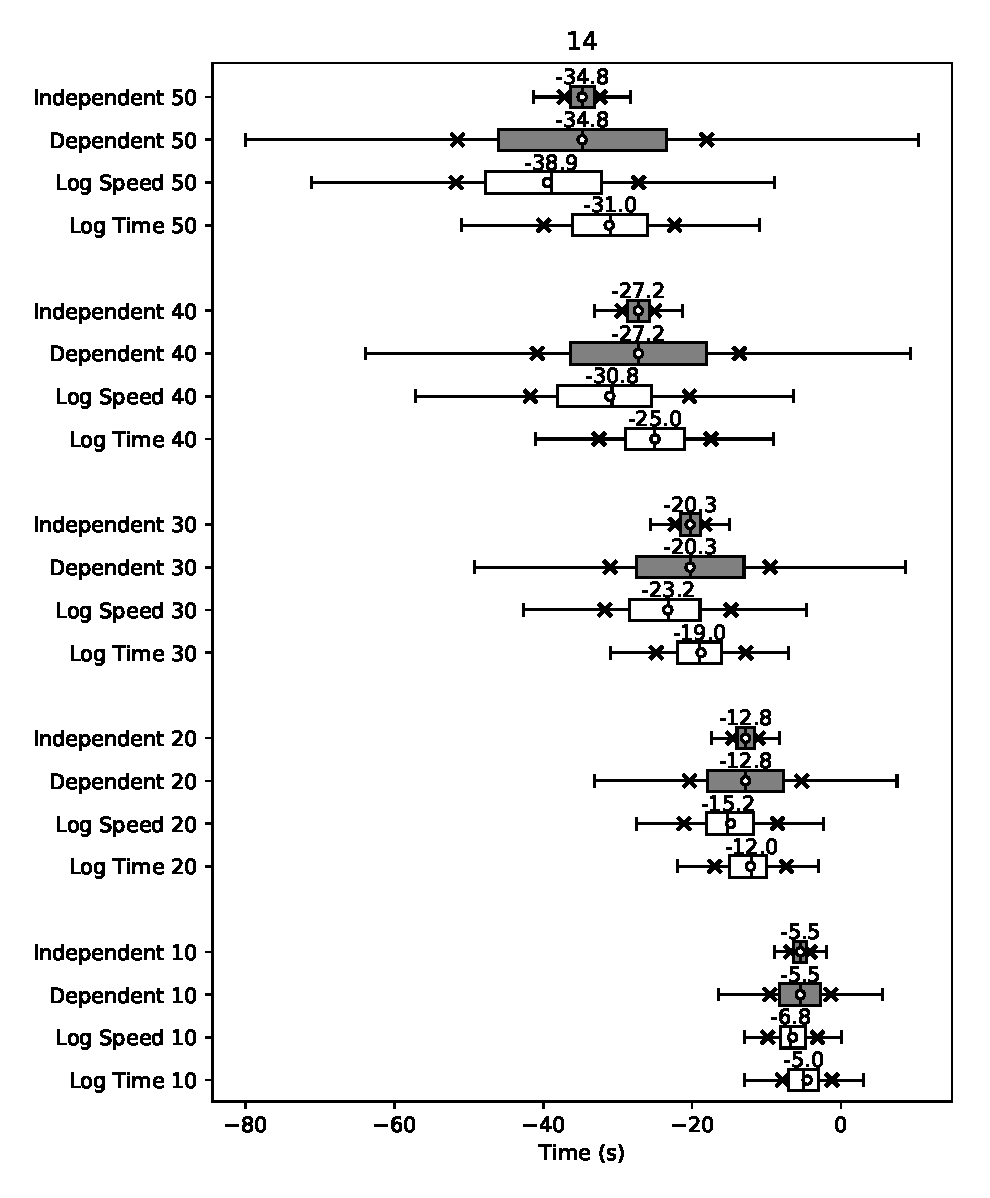
\includegraphics[scale=0.7]{14.eps}
					\caption{Result of prediction and actual values when cross referencing data. Same point used as in figure \ref{fig:box1}}
					\label{fig:cross1}
				\end{figure}

	\section{Discussion}
%		Taking HybridP data as gospel
		This entire results of this thesis build on the data collected by the Mobilaris Hybrid Positioning system, which is not flawless. This is something which has always been taken into consideration when dealing with the logs produced. Sometimes there are big jumps in space or time, often adjacent logs are not adjacent in the mine graph, and sometimes a vehicle travelling at full speed will appear to be standing still for a second or two if one were to only observe the coordinates. However most of the time the system is functioning perfectly fine, estimated at 90-95\% according to the developers. However, these studies are not made public, which is a downside. Assuming the developers are right around 95\% of the logs are good to use and anything else is either filtered out or simply produces some noise and outliers in the final results. Some data might be offset an edge forwards or backward since the positioning might be off sometimes. This is fine for most cases since most adjacent road segments ought to have somewhat similar distributions. Although, in places like corners or intersections, where rapid velocity change can occur between edges, this might create an undue higher variance. In addition, there's the question if the velocity a log reports should be applied to the upcoming edge or the preceding one. It might be the case that in reality this would be random chance if the vehicle positioning happened to be just inside the radius of being reported on one node instead of the next. This issue was resolved by simply picking the preceding edge as the assumed correct answer cos that makes sense if you have to explain your reasoning to someone.

		In addition, the predictions made by this solution are all based on the values of speed logged by the Hybrid Positioning system. If these values do not correspond well to the actual speed and time taken by the car to traverse a path then there's nothing this solution can do about it. Using Log Time to calculate a velocity distribution, by dividing the distance of an edge by the time taken to traverse it, would be hard to implement. As logs in the Hybrid Positioning system are always produced once per second this is the only granularity available. If a vehicle travels 7.5m/s  it will end up in-between nodes at the point of logging, and its position will snap to the closest node. Calculating speed from this would result in one log reporting 5m/s, while the next log reports 10m/s. Over several logs this will of course even out, but for the sake of determining velocity over a singular edge this is not well suited.

		%Addition of edge speeds are not independent.
		The dependency of adjacent edge speeds seems to lean quite heavily towards dependence. Absolute dependency, as shown in the results, seems to produce a slightly too high variance, however, and the truth is most likely less extreme than absolute dependence. It is likely the case that the dependency of adjacent edges varies depending on the edges involved. It might be the case that roads with very little traffic have high dependence, as drivers can hold whatever speed they wish without disturbance, while heavily trafficked roads would have more independent edge speeds. Further research would need to be done in order to find things like this out. Finding out the speed dependence of adjacent edges can result in more accurate prediction. It is then also possible to take the current speed of a vehicle into account when predicting speed over upcoming edges, and in doing so greatly reduce the variance of the prediction. Tests would need to prove the accuracy of such a prediction.

		%Distributions over edges not all normally distributed.
		It is also obvious that the distributions of velocities across edges are not always entirely Gaussian distributed. Assuming that they are Gaussian can both inflate or deflate variance, depending on the actual distribution. As seen in section \ref{sec:dependenceResults} the actual distributions can deviate quite a lot in some cases, and introduce error as a consequence. The final results can still appear to be normal distributed, as adding and subtracting multiple distributions together tend towards a normal distribution regardless. The way by which one ends up with a normal distributed result in the algorithm, however, is through simplification and linearisation, and so variance and mean is not necessarily the same.

		The linearisation does not seem to be very detrimental, and the variance of dependent theory seems to be slightly high even when not linearising.

		%Lack of data over an edge is no problem, as data will grow with time.
		It's notable that a vast amount of edges had too few data points to create a proper velocity distribution. As time passes more and more data can be collected and this problem is solved on its own. The results show that old data suffices, and it is vastly superior to no data. Low amounts of data seem to lead to higher variance. This is most likely the cause of outliers having a greater influence on the distributions used for predictions.

		If there is any change in the mine road conditions, network or workflow, however, old data can become obsolete and misguiding. One can also reason that the more travelled a mine section is the more important it is to have accurate predictions. And so the most important mine segments will inherently have a lot of data to base predictions on.

		A consequence of drivers being given access to predictions like those in this thesis might be a change in driving behaviour. Might be that when drivers are made aware of the chances to make it to a meeting slot that they would speed up to increase their chances, and so a collection of data would form at the upper end of speed records.

		Another idea would be for mine management to mandate a speed at which vehicles travel at, and so greatly reduce the variance of predictions leading to less uncertainty in predictions. Subdividing logs into more specific categories could also reduce variance, such as per vehicle, time of day, driver, and any sort of conditions which might occur, such as a truck being loaded or not, a state of emergency having been issued, etc.

		An ethical dilemma might present itself in extensively logging and analysing driving patterns, however. It could be seen as an invasion of privacy for a mining company to map out the movement of its employees and contractors. Such an issue could be mitigated somewhat by grouping vehicles together in categories, such as loaders, trucks, drills, etc. Even so, the issue can arise again if the number of drivers in a given category is very small, or even just one.

		On the other hand, if stress or other health risks due to the possibility or occurrence of collisions are major factors it might prove unethical to not use a solution which mitigates these factors if one exists. Including positioning of people in the mine and arrival estimations to them could also serve as a major safety feature to help ensure employee safety in a mine. Mappings of behaviour can also detect high-risk areas where drivers tend to exceed speed limits, allowing measures to be put in place to reduce speeds and increase safety.

		For vehicles to have a predetermined destination, known to the system, is an optional variable. Disregarding it would create a more general solution, in which drivers can embark on their journey without any preparations, and could even accommodate vehicles which do not use the solution algorithm. Having destinations known however can reduce guess-work a lot, produce more optimal solutions and simplify computation. For this reason, this thesis assumes that such knowledge exists.

		This thesis has tried to not specify the exact technology or setup required to produce the solution, and in such a way keep it as general as possible and able to be applied to a variety of setups. Although the mines of today often use a central server to orchestrate communication and positioning the mines of the future might implement more peer to peer or decentralized networks, and so the suggested solution is designed to still work regardless.

		If more accurate positioning is used for logging the question arises of how granular the assignments of velocity probability distributions should be to still be useful. The current granularity of five meters could feel a bit coarse, however, a granularity of one centimeter would be absurd. The proper answer to this question remains to be answered and might differ depending on mine, mine-section, use case, performance needs, or others. The granularity in this thesis was set based on limitations and nothing else.

		The presented solution seems to give reliable predictions in the dependent case, that err somewhat on the side of caution. Implementing the solution of basic predictions as it is could provide drivers with information of when they need to diverge to make way for oncoming traffic well ahead of time, and so hopefully provide simple but efficient traffic control in an underground mine. The solution could also be used to predict when and where two vehicles will meet in a mine by searching for nodes in which the expected time difference is as close to zero as possible, and so give the driver better awareness of their surroundings. The degree to which a system chooses to inform versus direct a driver based upon the results of this solution is up to the implementation itself.

    \section{Conclusion}
		The purpose of this thesis was to produce a predictive model for traffic management in a mine. This was done using statistics and historical travel logs to predict difference in arrival time to a point. It can be concluded that although not perfect, predicting the difference in arrival time for two vehicles to a point is very much doable and could be used today to predict collisions. The results of this master's thesis show that the predictions correspond quite well to actual real world logs. Compared to drivers having no awareness at all, or only knowing rough positions of surrounding vehicles, this solution could improve driver safety and efficiency in a mine.

		Managing inaccurate positioning, connection loss, and more complex cases are addressed in theory, but have no real-world data to be test against.

        \subsection{Future work}
			There are three main ways in the eyes of the author how to improve the predictions of this thesis.
			\begin{itemize}
				\item Improve the correlation between Log Time and Log Speed. The prediction is trying to mimic Log Speed, and if Log Speed is not in line with Log Time then accurate results can never be obtained.
				\item Allow the theoretical model to deviate from the assumption that all distributions are Gaussian distributed. For instance by modelling velocity distributions with a mixture model, and not linearising division.
				\item Find appropriate dependency coefficients. This might vary depending on mine, location, vehicle type and other variables.
			\end{itemize}

			Given more data in logs, such as when two vehicles meet, when a collision occurs and a vehicle is forced to reverse, network disconnections, as well as simultaneously gather logs from systems with different accuracies more tests of the suggested solution can be performed. Such tests can then be grounded in reality, instead of being speculative or simulations.

			It might be necessary to study individual types of vehicles as well. Small personnel transports might have entirely different driving patterns to heavy trucks or machinery, and as such might present entirely different problems that need to be dealt with.

			Seeing an actual implementation of the suggested solution algorithm and evaluation of how it affects driver safety, traffic flow and driver stress/satisfaction is an important next step for this solution.
	\printbibliography

\end{document}
